% forallxyyc-html
% Driver file to produce HTML etc. version of forall x:YYC 
% using LaTeXML 

\documentclass{book}

\RequirePackage{xcolor,tabularx}
\definecolor{lyallpink}{RGB}{222,31,149}
\colorlet{leadbeater}{lyallpink}
\colorlet{dkleadbeater}{lyallpink!80!black}
\colorlet{ltleadbeater}{lyallpink!50}
\colorlet{vltleadbeater}{lyallpink!3}

\usepackage{forallxyyc-style}
\usepackage{forallxyyc}

\title{forall x: Calgary\\
An Introduction to Formal Logic}

\author{P.~D. Magnus\\
Tim Button\\
\textit{with additions by}\\
J.~Robert Loftis\\
Robert Trueman\\
\textit{remixed and revised by}\\
Aaron Thomas-Bolduc\\
Richard Zach}

\date{\forallxversion}


\begin{document}

\maketitle

\frontmatter

\ifHTMLtarget
  \tableofcontents
  %!TEX root = forallxyyc.tex

\ifHTMLtarget\else
% Bastard Title

\pagestyle{empty}

\vspace*{80pt}

\begin{raggedleft}
\fontsize{30pt}{24pt}\sffamily
\selectfont
  \textbf{forall 
  {\fontsize{37pt}{24pt}\selectfont\rmfamily\textit{x}}: 
  Calgary}

\medskip\fontsize{18pt}{20pt}\selectfont

\textbf{An Introduction to\\ Formal Logic}

\vfill
\fontsize{12pt}{16pt}\selectfont \textit{By } \textbf{P.~D. Magnus}\\
\textbf{Tim Button}\\
\textit{with additions by}\\
\textbf{J.~Robert Loftis}\\
\textbf{Robert Trueman}\\
\textit{remixed and revised by}\\
\textbf{Aaron Thomas-Bolduc}\\ \textbf{Richard Zach}

\vfill
\textbf{\forallxversion}\par
\end{raggedleft}

\newpage

\noindent\small%
\fi
This book is based on
\href{https://www.homepages.ucl.ac.uk/~uctytbu/OERs.html}{\forallx:
\textit{Cambridge}}, by 
\href{https://www.homepages.ucl.ac.uk/~uctytbu/}{Tim Button} (University College London), 
used under a \href{https://creativecommons.org/licenses/by/4.0/}{CC BY
4.0} license, which is based in turn
on \href{https://www.fecundity.com/logic/}{\forallx}, by
\href{https://www.fecundity.com/job/}{P.D.\ Magnus} 
(University at Albany, State University of New York),
used under a \href{https://creativecommons.org/licenses/by/4.0/}{CC BY
4.0} license, 
and was remixed, revised, \& expanded by Aaron
Thomas-Bolduc \& \href{https://richardzach.org/}{Richard Zach}
(University of Calgary).
It includes additional material from \forallx{} by P.~D. Magnus and
\href{https://www.homepages.ucl.ac.uk/~uctytbu/OERs.html}{\textit{Metatheory}} by Tim Button, 
used under a \href{https://creativecommons.org/licenses/by/4.0/}{CC BY
4.0} license, 
from \href{https://github.com/rob-helpy-chalk/openintroduction}{\forallx: \textit{Lorain
County Remix}},
by \href{https://sites.google.com/site/cathalwoods/}{Cathal Woods} and
J. Robert Loftis, and from \href{http://www.rtrueman.com/uploads/7/0/3/2/70324387/modal_logic_primer.pdf}{\textit{A Modal Logic Primer}} by \href{http://www.rtrueman.com/}{Robert Trueman}, used with permission.


\ifHTMLtarget\else
  \bigskip

  \noindent\footnotesize
\fi
This work is licensed under a \href{https://creativecommons.org/licenses/by/4.0/}{Creative Commons Attribution 4.0} license.
You are free to copy and redistribute the material in any medium or format, and  remix, transform, and build upon the material for any purpose, even commercially, under the following terms:
\begin{itemize}
\item You must give appropriate credit, provide a link to the license, and indicate if changes were made. You may do so in any reasonable manner, but not in any way that suggests the licensor endorses you or your use.
\item You may not apply legal terms or technological measures that legally restrict others from doing anything the license permits.
\end{itemize}

\ifHTMLtarget\else
\vfil\normalsize\noindent
\fi
The \LaTeX{} source for this book is available on Github at
\href{https://github.com/rzach/forallx-yyc/}{github.com/rzach/forallx-yyc/} and in PDF and
HTML format at
\href{https://forallx.openlogicproject.org}{forallx.openlogicproject.org}.
This version is revision \gitAbbrevHash{}
(\gitAuthorDate).

\bigskip
\noindent
The preparation of this textbook was made possible by a grant from the \href{https://taylorinstitute.ucalgary.ca/}{Taylor Institute for Teaching and Learning}.

\bigskip
\noindent
\href{https://taylorinstitute.ucalgary.ca/}{\includegraphics[width=8cm]{assets/ti-color}}

\ifHTMLtarget
The HTML format is produced using
\href{https://vlmantova.github.io/bookml/}{BookML} by
\href{https://eps.leeds.ac.uk/maths/staff/4058/dr-vincenzo-l-mantova}{Vincenzo Mantova}
and \href{https://dlmf.nist.gov/LaTeXML/}{\LaTeX{}ML} by
\href{https://www.nist.gov/people/bruce-r-miller}{Bruce Miller} and
\href{https://prodg.org/}{Deyan Ginev}. 
\else
\bigskip
\noindent Cover design by Mark Lyall.
\fi

\else
  %!TEX root = forallxyyc.tex

\ifHTMLtarget\else
% Bastard Title

\pagestyle{empty}

\vspace*{80pt}

\begin{raggedleft}
\fontsize{30pt}{24pt}\sffamily
\selectfont
  \textbf{forall 
  {\fontsize{37pt}{24pt}\selectfont\rmfamily\textit{x}}: 
  Calgary}

\medskip\fontsize{18pt}{20pt}\selectfont

\textbf{An Introduction to\\ Formal Logic}

\vfill
\fontsize{12pt}{16pt}\selectfont \textit{By } \textbf{P.~D. Magnus}\\
\textbf{Tim Button}\\
\textit{with additions by}\\
\textbf{J.~Robert Loftis}\\
\textbf{Robert Trueman}\\
\textit{remixed and revised by}\\
\textbf{Aaron Thomas-Bolduc}\\ \textbf{Richard Zach}

\vfill
\textbf{\forallxversion}\par
\end{raggedleft}

\newpage

\noindent\small%
\fi
This book is based on
\href{https://www.homepages.ucl.ac.uk/~uctytbu/OERs.html}{\forallx:
\textit{Cambridge}}, by 
\href{https://www.homepages.ucl.ac.uk/~uctytbu/}{Tim Button} (University College London), 
used under a \href{https://creativecommons.org/licenses/by/4.0/}{CC BY
4.0} license, which is based in turn
on \href{https://www.fecundity.com/logic/}{\forallx}, by
\href{https://www.fecundity.com/job/}{P.D.\ Magnus} 
(University at Albany, State University of New York),
used under a \href{https://creativecommons.org/licenses/by/4.0/}{CC BY
4.0} license, 
and was remixed, revised, \& expanded by Aaron
Thomas-Bolduc \& \href{https://richardzach.org/}{Richard Zach}
(University of Calgary).
It includes additional material from \forallx{} by P.~D. Magnus and
\href{https://www.homepages.ucl.ac.uk/~uctytbu/OERs.html}{\textit{Metatheory}} by Tim Button, 
used under a \href{https://creativecommons.org/licenses/by/4.0/}{CC BY
4.0} license, 
from \href{https://github.com/rob-helpy-chalk/openintroduction}{\forallx: \textit{Lorain
County Remix}},
by \href{https://sites.google.com/site/cathalwoods/}{Cathal Woods} and
J. Robert Loftis, and from \href{http://www.rtrueman.com/uploads/7/0/3/2/70324387/modal_logic_primer.pdf}{\textit{A Modal Logic Primer}} by \href{http://www.rtrueman.com/}{Robert Trueman}, used with permission.


\ifHTMLtarget\else
  \bigskip

  \noindent\footnotesize
\fi
This work is licensed under a \href{https://creativecommons.org/licenses/by/4.0/}{Creative Commons Attribution 4.0} license.
You are free to copy and redistribute the material in any medium or format, and  remix, transform, and build upon the material for any purpose, even commercially, under the following terms:
\begin{itemize}
\item You must give appropriate credit, provide a link to the license, and indicate if changes were made. You may do so in any reasonable manner, but not in any way that suggests the licensor endorses you or your use.
\item You may not apply legal terms or technological measures that legally restrict others from doing anything the license permits.
\end{itemize}

\ifHTMLtarget\else
\vfil\normalsize\noindent
\fi
The \LaTeX{} source for this book is available on Github at
\href{https://github.com/rzach/forallx-yyc/}{github.com/rzach/forallx-yyc/} and in PDF and
HTML format at
\href{https://forallx.openlogicproject.org}{forallx.openlogicproject.org}.
This version is revision \gitAbbrevHash{}
(\gitAuthorDate).

\bigskip
\noindent
The preparation of this textbook was made possible by a grant from the \href{https://taylorinstitute.ucalgary.ca/}{Taylor Institute for Teaching and Learning}.

\bigskip
\noindent
\href{https://taylorinstitute.ucalgary.ca/}{\includegraphics[width=8cm]{assets/ti-color}}

\ifHTMLtarget
The HTML format is produced using
\href{https://vlmantova.github.io/bookml/}{BookML} by
\href{https://eps.leeds.ac.uk/maths/staff/4058/dr-vincenzo-l-mantova}{Vincenzo Mantova}
and \href{https://dlmf.nist.gov/LaTeXML/}{\LaTeX{}ML} by
\href{https://www.nist.gov/people/bruce-r-miller}{Bruce Miller} and
\href{https://prodg.org/}{Deyan Ginev}. 
\else
\bigskip
\noindent Cover design by Mark Lyall.
\fi

  \clearpage
  \pagestyle{leadbeater}
  \thispagestyle{plain}
  \currentpdfbookmark{Table of Contents}{name}
  \tableofcontents*
\fi

\chapter{Preface}

As the title indicates, this is a textbook on formal logic.  Formal logic concerns the study of a certain kind of language which, like any language, can serve to express states of affairs.  It is a formal language, i.e., its expressions (such as sentences) are defined formally.  This makes it a very useful language for being very precise about the states of affairs its sentences describe. In particular, in formal logic it is impossible to be ambiguous. The study of these languages centres on the relationship of entailment between sentences, i.e., which sentences follow from which other sentences.  Entailment is central because by understanding it better we can tell when some states of affairs must obtain provided some other states of affairs obtain.  But entailment is not the only important notion. We will also consider the relationship of being satisfiable, i.e., of not being mutually contradictory.  These notions can be defined semantically, using precise definitions of entailment based on interpretations of the language---or proof-theoretically, using formal systems of deduction.

Formal logic is of course a central sub-discipline of philosophy, where the logical relationship of assumptions to conclusions reached from them is important.  Philosophers investigate the consequences of definitions and assumptions and evaluate these definitions and assumptions on the basis of their consequences. It is also important in mathematics and computer science. In mathematics, formal languages are used to describe not ``everyday'' states of affairs, but mathematical states of affairs. Mathematicians are also interested in the consequences of definitions and assumptions, and for them it is equally important to establish these consequences (which they call ``theorems'') using completely precise and rigorous methods. Formal logic provides such methods.  In computer science, formal logic is applied to describe the state and behaviours of computational systems, e.g., circuits, programs, databases, etc.  Methods of formal logic can likewise be used to establish consequences of such descriptions, such as whether a circuit is error-free, whether a program does what it's intended to do, whether a database is consistent or if something is true of the data in it.

The book is divided into nine parts. Part~\ref{ch.intro} introduces the topic and notions of logic in an informal way, without introducing a formal language yet.  Parts \ref{ch.TFL}--\ref{ch.NDTFL} concern truth-functional languages. In it, sentences are formed from basic sentences using a number of connectives (`or', `and', `not', `if \dots then') which just combine sentences into more complicated ones.  We discuss logical notions such as entailment in two ways: semantically, using the method of truth tables (in Part~\ref{ch.TruthTables}) and proof-theoretically, using a system of formal derivations (in Part~\ref{ch.NDTFL}).  Parts \ref{ch.FOL}--\ref{ch.NDFOL} deal with a more complicated language, that of first-order logic. It includes, in addition to the connectives of truth-functional logic, also names, predicates, identity, and the so-called quantifiers. These additional elements of the language make it much more expressive than the truth-functional language, and we'll spend a fair amount of time investigating just how much one can express in it.  Again, logical notions for the language of first-order logic are defined semantically, using interpretations, and proof-theoretically, using a more complex version of the formal derivation system introduced in Part~\ref{ch.NDTFL}.  Part~\ref{ch.ML} discusses the extension of TFL by non-truth-functional operators for possibility and necessity: modal logic. Part~\ref{ch.normalform} covers two advanced topics: that of conjunctive and disjunctive normal forms and the functional completeness of the truth-functional connectives, and the soundness of natural deduction for TFL.

In the appendices you'll find a discussion of alternative notations for the languages we discuss in this text, of alternative derivation systems, and a quick reference listing most of the important rules and definitions. The central terms are listed in a glossary at the very end.

\paragraph{Credits} This book is based on a text originally written by P.~D. Magnus in the version revised and expanded by Tim Button. It also includes some material (mainly exercises) by J.~Robert Loftis. The material in Part~\ref{ch.ML} is based on notes by Robert Trueman (but rewritten to use Fitch's original natural deduction rules for modal logic), and the material in chapters~\ref{c:NormalForms}, \ref{c:FunctionalCompleteness}, and~\ref{ch:Soundness} on two chapters from Tim Button's open text \emph{Metatheory}. Aaron Thomas-Bolduc and Richard Zach have combined elements of these texts into the present version, changed some of the terminology and examples, rewritten some sections, and added material of their own.  In particular, Richard Zach rewrote chapters \ref{s:Arguments} and~\ref{s:Valid}, and added chapters \ref{s:AbmbiguityTFL}, \ref{s:stratTFL}, \ref{s:ambiguityFOL}, and~\ref{ch:equivalences}. As of the Fall 2019 edition, the part on FOL uses the syntax more common in advanced texts (such as those based on the Open Logic Project) where arguments to predicate symbols are enclosed in parentheses (i.e., `$R(a,b)$' instead of `$Rab$'). The resulting text is licensed under a Creative Commons Attribution 4.0 license. There are \href{https://github.com/OpenLogicProject/OpenLogic/wiki/Other-Logic-Textbooks}{several other} ``remixes'' of \emph{forall x}, including translations of this version.

\paragraph{Notes for instructors} The material in this book is suitable for a semester-long introduction to formal logic. I cover parts \ref{ch.intro}--\ref{ch.NDFOL} plus chapters \ref{c:NormalForms}, \ref{c:FunctionalCompleteness}, and \ref{ch:equivalences} in 12 weeks, although I leave out partial truth tables and derived inference rules.

The most recent version of this book is available in PDF at \href{https://forallx.openlogicproject.org}{forallx.openlogicproject.org}, but changes frequently.  The CC BY license gives you the right to download and distribute the book yourself. In order to ensure that all your students have the same version of the book throughout the term you're using it, you should do so: upload the PDF you decide to use to your LMS rather than merely give your students the link. You are also free to have the PDFs printed by your bookstore, but some bookstores will be able to purchase and stock the softcover books available on Amazon.

Note that solutions to many exercises in the book are available at the above site as well (to everyone, including your students).

The syntax and proof systems (except those for modal logic) are supported by Graham Leach-Krouses's free, online logic teaching software application \emph{Carnap} (\href{https://carnap.io}{carnap.io}). This allows for submission and automated marking of exercises such as symbolization, truth tables, and natural deduction proofs.  Instructors on carnap.io will be able to find \href{https://carnap.io/shared/rzach@ucalgary.ca/forall%20x:%20Calgary.md}{samples of additional exercises} they may wish to adapt or assign as-is.

\mainmatter

\input{forallx-yyc-what}
\input{forallx-yyc-tfl}
\input{forallx-yyc-truthtables}
\input{forallx-yyc-prooftfl}
\input{forallx-yyc-fol}
%!TEX root = forallxyyc.tex
\part{Interpretations}
\label{ch.semantics}
\addtocontents{toc}{\protect\mbox{}\protect\hrulefill\par}


\chapter{Extensionality}\label{s:Interpretations}

Recall that TFL is a truth-functional language. Its connectives are all truth-functional, and \emph{all} that we can do with TFL is key sentences to particular truth values. We can do this \emph{directly}. For example, we might stipulate that the TFL sentence `$P$' is to be true. Alternatively, we can do this \emph{indirectly}, offering a symbolization key, e.g.:
	\begin{ekey}
		\item[P] Big Ben is in London.
	\end{ekey}
 But recall from \S\ref{s:TruthFunctionality} that this is \emph{just} a means of specifying `$P$'s truth value; the symbolization key statement amounts to something like the following stipulation: 
	\begin{itemize}
		\item The TFL sentence `$P$' is true \ifeff{} Big Ben is in London.
	\end{itemize}
And we emphasized in \S\ref{s:TruthFunctionality} that TFL cannot handle differences in meaning that go beyond mere differences in truth value.

\section{Symbolizing versus translating}

FOL has some similar limitations. It gets beyond mere truth values, since it enables us to split up sentences into terms, predicates and quantifiers. This enables us to consider what is \emph{true of} some particular object, or of some or all objects. \emph{But that's it}.

To unpack this a bit, consider this symbolization key: 
	\begin{ekey}
		\item[\atom{C}{x}] \gap{x} teaches Logic III in Calgary
	\end{ekey} 
This stipulation does not carry the \emph{meaning} of the English predicate across into our FOL predicate. We are simply stipulating something like this:
	\begin{itemize}
		\item `$\atom{C}{x}$' and `\gap{x} teaches Logic III in Calgary' are to be \emph{true of} exactly the same things.
	\end{itemize}
So, in particular:
	\begin{itemize}
		\item `$\atom{C}{x}$' is to be true of exactly those things which teach Logic III in Calgary (whatever those things might be).
	\end{itemize}
This is an indirect way of stipulating which things a predicate is true of.

Alternatively, we can stipulate predicate extensions directly. For example, we can stipulate that `$\atom{C}{x}$' is to be true of Richard Zach, and Richard Zach alone. As it happens, this direct stipulation would have the same effect as the indirect stipulation, since Richard, and Richard alone, teaches Logic~III in Calgary. Note, however, that the English predicates `\blank\ is Richard Zach' and `\blank\ teaches Logic III in Calgary' have very different meanings!

The point is that FOL has no resources for dealing with nuances of meaning. When we interpret FOL, all we are considering is what the predicates are true of, regardless of whether we specify these things directly or indirectly. The things a predicate is true of are known as the \define{extension} of that predicate. We say that FOL is an \define{extensional language} because FOL does not represent differences of meaning between predicates that have the same extension.    

This is why we speak of \emph{symbolizing} English sentences in FOL. It is doubtful that we are \emph{translating} English into FOL, for translation should preserve meaning.

\section{Extensions}\label{sec:extensions}
We can stipulate directly what predicates are to be true of. And our stipulations can be as arbitrary as we like. For example, we could stipulate that `$\atom{H}{x}$' should be true of, and only of, the following objects:
	\begin{itemize}
		\item Justin Trudeau
		\item the number $\pi$
		\item every top-F key on every piano ever made
	\end{itemize}
Armed with this interpretation of `$\atom{H}{x}$', suppose we now add to our symbolization key:
	\begin{ekey}
		\item[j] Justin Trudeau
		\item[a] Angela Merkel
		\item[p] the number $\pi$
	\end{ekey}
Then `$\atom{H}{j}$' and `$\atom{H}{p}$' will both be true, on this interpretation, but `$\atom{H}{a}$' will be false, since Angela Merkel was not among the stipulated objects.

This process of explicit stipulation is sometimes described as stipulating the \emph{extension} of a predicate. Note that, in the stipulation we just gave, the objects we listed have nothing particularly in common. This doesn't matter. Logic doesn't care about what we humans (at a particular moment) think `naturally goes together'; to logic, all objects are on an equal footing.

Any well-defined collection of objects is a potential extension of a one-place predicate.  The example above shows one way of stipulating the extension of `$\atom{H}{x}$' by \emph{enumeration}, i.e., we simply list the objects in the extension of~`$\atom{H}{x}$'. We can also stipulate the extension, as we have also already seen, by giving an English predicate, such as `\gap{x} teaches Logic~III at Calgary' or `\gap{x} is an even integer between $3$ and $9$'. The latter would specify an extension consisting of, and only of, $4$, $6$, and~$8$.

Note that some predicates of English, such as `\gap{x} is a round square', are not true of anything.  In this case we say the extension of the predicate is \emph{empty}.  We do allow empty extensions, and we can stipulate that the extension of `$\atom{H}{x}$' is to be empty simply by not listing any members. (It may be odd to consider collections of no things, but logic is odd this way sometimes.)


\section{Many-place predicates}
All of this is quite easy to understand when it comes to one-place predicates, but it gets messier when we deal with two-place predicates. Consider a symbolization key like:
	\begin{ekey}
		\item[\atom{L}{x,y}] \gap{x} loves \gap{y}
	\end{ekey}
Given what we said above, this symbolization key should be read as saying:
	\begin{itemize}
		\item `$\atom{L}{x,y}$' and `\gap{x} loves \gap{y}' are to be true of exactly the same things.
	\end{itemize}
So, in particular:
	\begin{itemize}
		\item `$\atom{L}{x,y}$' is to be true of x and y (in that order) \ifeff{} x loves y.
	\end{itemize}
It is important that we insist upon the order here, since love---famously---is not always reciprocated. (Note that `x' and `y' on the right here are symbols of augmented English, and that they are being \emph{used}. By contrast, `$x$' and `$y$' in `$\atom{L}{x,y}$' are symbols of FOL, and they are being \emph{mentioned}.)

That is an indirect stipulation. What about a direct stipulation? This is also tricky. If we \emph{simply} list objects that fall under `$\atom{L}{x,y}$', we will not know whether they are the lover or the beloved (or both). We have to find a way to include the order in our explicit stipulation.

To do this, we can specify that two-place predicates are true of \emph{pairs} of objects, where the order of the pair is important. Thus we might stipulate that `$\atom{B}{x,y}$' is to be true of, and only of, the following pairs of objects:
	\begin{itemize}
		\item \ntuple{Lenin, Marx}
		\item \ntuple{de Beauvoir, Sartre}
		\item \ntuple{Sartre, de Beauvoir}
	\end{itemize}
Here the angle-brackets keep us informed concerning order. Suppose we now add the following stipulations:
	\begin{ekey}
		\item[l] Lenin
		\item[m] Marx
		\item[b] de Beauvoir
		\item[r] Sartre
	\end{ekey}
Then `$\atom{B}{l,m}$' will be true, since \ntuple{Lenin, Marx} is in our explicit list, but `$\atom{B}{m,l}$' will be false, since \ntuple{Marx, Lenin} is not in our list. However, both `$\atom{B}{b,r}$' and `$\atom{B}{r,b}$' will be true, since both \ntuple{de Beauvoir, Sartre} and \ntuple{Sartre, de Beauvoir} are in our explicit list.

To make these ideas more precise, we would need to develop some very elementary \emph{set theory}. Set theory has formal apparatus which allows us to deal with extensions, ordered pairs, and so forth. However, set theory is not covered in this book. So I shall leave these ideas at an imprecise level. Nevertheless, the general idea should be clear.


\section{Semantics for identity}
Identity is a special predicate of FOL. We write it a bit differently than other two-place predicates: `$x=y$' instead of `$\atom{I}{x,y}$' (for example). More important, though, is that its interpretation is fixed, once and for all.

If two names refer to the same object, then swapping one name for another will not change the truth value of any sentence. So, in particular, if `$a$' and `$b$' name the same object, then all of the following will be true:\label{model.nonidentity}
	\begin{align*}
	 	\atom{A}{a} &\eiff \atom{A}{b} \\
	 	\atom{B}{a} &\eiff \atom{B}{b}\\
		\atom{R}{a,a} &\eiff \atom{R}{b,b}\\
		\atom{R}{a,a} & \eiff \atom{R}{a,b}\\
		\atom{R}{c,a} &\eiff \atom{R}{c,b}\\
		\forall x\, \atom{R}{x,a} &\eiff \forall x\, \atom{R}{x,b}
	\end{align*}
Some philosophers have believed the reverse of this claim. That is, they have believed that when exactly the same sentences (not containing `$=$') are true of $a$ and $b$, then $a$ and $b$ are the very same object. This is a highly controversial philosophical claim---sometimes called the \emph{identity of indiscernibles}---and our logic will not subscribe to it; we allow that exactly the same things might be true of two \emph{distinct} objects.  

To bring this out, consider the following interpretation:
	\begin{ekey}
		\item[\text{domain}] P.~D.\ Magnus, Tim Button
		\item[a] P.~D.\ Magnus
		\item[b] Tim Button
		\item[\atom{\metav{R}}{x_1,\dots, x_n}] For every primitive
		predicate \metav{R} we care to consider, that predicate is true of
		\emph{nothing}.
	\end{ekey}
Suppose `$A$' is a one-place predicate; then `$\atom{A}{a}$' is false and `$\atom{A}{b}$' is false, so `$\atom{A}{a} \eiff \atom{A}{b}$' is true. Similarly, if `$R$' is a two-place predicate, then `$\atom{R}{a,a}$' is false and `$\atom{R}{a,b}$' is false, so that `$\atom{R}{a,a} \eiff \atom{R}{a,b}$' is true. And so it goes: every atomic sentence not involving `$=$' is false, so every biconditional linking such sentences is true. For all that, Tim Button and P.~D.\ Magnus are two distinct people, not one and the same!

\section{Interpretations}
We defined a \define{valuation} in TFL as any assignment of truth and falsity to sentence letters. In FOL, we are going to define an \define{interpretation} as consisting of four things:
	\begin{compactlist}
		\item the specification of a domain;
		\item for each sentence letter we care to consider, a truth value;
		\item for each name that we care to consider, an assignment of exactly one object within the domain;
		\item for each predicate that we care to consider (apart from
		`$=$'), a specification of what things (in what order) the
		predicate is to be true of.
	\end{compactlist}
We don't need to specify anything for`$=$', since it has a
\emph{fixed} meaning, namely that of identity. Everything is identical
to itself, and only to itself. 

The symbolization keys that we considered in Part~\ref{ch.FOL} consequently give us one very convenient way to present an interpretation. We will continue to use them in this chapter. Following the discussion of \S\ref{sec:extensions}, we now also allow extensions specified by enumerations on the right side, e.g.,
\begin{ekey}
	\item[\text{domain}] heads of state, numbers
	\item[\atom{H}{x}] Justin Trudeau, Angela Merkel, $\pi$
\end{ekey}
is a perfectly good way of specifying an interpretation, as is
\begin{ekey}
	\item[\text{domain}] $0$, $1$, $2$
	\item[\atom{L}{x,y}] \ntuple{$0$,$1$}, \ntuple{$0$, $2$}, \ntuple{$1$, $2$}
\end{ekey}
We could have specified the same extension (on this particular domain) by giving the English predicate `\gap{x} is less than \gap{y}'.


\newglossaryentry{interpretation}{
  name = {interpretation},
  description = {A specification of a \gls{domain} together with the objects the \glspl{name} pick out and which objects the \glspl{predicate} are true of}
}

However, it is sometimes also convenient to present an interpretation \emph{diagrammatically}. To illustrate (literally): suppose we want to consider just a single two-place predicate, `$\atom{R}{x,y}$'. Then we can represent it just by drawing an arrow between two objects, and stipulate that `$\atom{R}{x,y}$' is to hold of $x$ and $y$ just in case there is an arrow running from $x$ to $y$ in our diagram. As an example, we might offer:
\begin{center}
\begin{bmlimage}
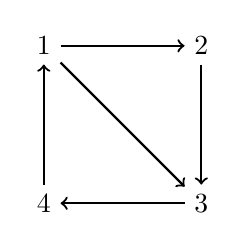
\begin{tikzpicture}
\node (atom1) at (0,2) {$1$};
\node (atom2) at (2,2) {$2$};
\node (atom3) at (2,0) {$3$};
\node (atom4) at (0,0) {$4$};
\draw[->, thick] (atom1)--(atom2);
\draw[->, thick] (atom2)--(atom3);
\draw[->, thick] (atom3)--(atom4);
\draw[->, thick] (atom4)--(atom1);
\draw[->, thick] (atom1) -- (atom3);
\end{tikzpicture}
\end{bmlimage}\bmlDescription{The numbers 1, 2, 3, and 4 are connected
by arrows. There are arrows from 1 to 2 and 3, from 2 to 3, from 3 to
4, and from 4 to 1.}
\end{center}
This diagram could be used to describe an interpretation whose domain is the first four positive whole numbers, and which interprets `$\atom{R}{x,y}$' as being true of and only of:
	\begin{center}
		\ntuple{$1$, $2$}, 
		\ntuple{$2$, $3$}, 
		\ntuple{$3$, $4$}, 
		\ntuple{$4$, $1$}, 
		\ntuple{$1$, $3$}
	\end{center}
Equally we might offer this diagram:

\begin{center}
\begin{bmlimage}
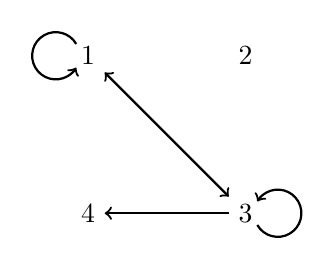
\begin{tikzpicture}
\node (atom1) at (0,2) {$1$};
\node (atom2) at (2,2) {$2$};
\node (atom3) at (2,0) {$3$};
\node (atom4) at (0,0) {$4$};
\draw[->, thick] (atom3)--(atom4);
\draw[->, thick] (atom1)+(-0.15,0.15) arc (-330:-30:.3); 
\draw[->, thick] (atom3)+(0.15,-0.15) arc (-150:150:.3); 
\draw[<->, thick] (atom1) -- (atom3);
\end{tikzpicture}
\end{bmlimage}\bmlDescription{The numbers 1, 3, and 4 are connected
by arrows. There are arrows from 1 to 3 and to itself, and from 3 to
1, 4 and itself. The number 2 is included but has no arrows coming in or going out.}
\end{center}

The interpretation specified by this diagram can also be given by listing what's in the domain and in the extension of~`$\atom{R}{x,y}$':
	\begin{ekey}
	\item[\text{domain}] $1$, $2$, $3$, $4$
	\item[R(x,y)] \ntuple{$1$, $3$}, 
		\ntuple{$3$, $1$}, 
		\ntuple{$3$, $4$}, 
		\ntuple{$1$, $1$},
		\ntuple{$3$, $3$}
	\end{ekey}
If we wanted, we could make our diagrams more complex. For example, we could add names as labels for particular objects. Equally, to symbolize the extension of a one-place predicate, we might simply draw a circle around some particular objects and stipulate that the thus encircled objects (and only them) are to fall under the predicate `$\atom{H}{x}$', say. To specify multiple predicates we could use colored (or dashed, dotted) lines for arrows and circles.


\chapter{Truth in FOL}\label{s:TruthFOL}
We have introduced you to interpretations. Since, among other things, they tell us which predicates are true of which objects, they will provide us with an account of the truth of atomic sentences. However, we now need to say, precisely, what it is for an arbitrary FOL sentence to be true or false in an interpretation.

We know from \S\ref{s:FOLSentences} that there are three kinds of sentence in FOL: 
	\begin{compactlist}
		\item atomic sentences,
		\item sentences whose main logical operator is a sentential connective,
		\item sentences whose main logical operator is a quantifier.
	\end{compactlist}
We need to explain truth for all three kinds of sentence.

We will provide a completely general explanation in this section. However, to try to keep the explanation comprehensible, we will, at several points, use the following interpretation:
	\begin{ekey}
		\item[\text{domain}] all people born before 2000 \textsc{ce}
		\item[a] Aristotle
		\item[b] Beyonc\'e
		\item[\atom{P}{x}] \gap{x} is a philosopher
		\item[\atom{R}{x,y}] \gap{x} was born before \gap{y}
	\end{ekey}
This will be our \emph{go-to example} in what follows.

\section{Atomic sentences}
The truth of atomic sentences should be fairly straightforward. For sentence letters, the interpretation specifies if they are true or false. The sentence `$\atom{P}{a}$' should be true just in case `$\atom{P}{x}$' is true of `$a$'. Given our go-to interpretation, this is true \ifeff{} Aristotle is a philosopher. Aristotle is a philosopher. So the sentence is true. Equally, `$\atom{P}{b}$' is false on our go-to interpretation.

Likewise, on this interpretation, `$\atom{R}{a,b}$' is true \ifeff{} the object named by `$a$' was born before the object named by `$b$'. Well, Aristotle was born before Beyonc\'e. So `$\atom{R}{a,b}$' is true. Equally, `$\atom{R}{a,a}$' is false: Aristotle was not born before Aristotle.

Dealing with atomic sentences, then, is very intuitive. When \metav{R} is an $n$-place predicate and $\metav{a}_1$, $\metav{a}_{2}$, \dots, $\metav{a}_{n}$ are names, 

	\factoidbox{
		The sentence $\atom{\metav{R}}{\metav{a}_{1},\metav{a}_{2},\dots,\metav{a}_{n}}$ is true in an interpretation \textbf{\ifeff}
		$\metav{R}$ is true of the objects named by $\metav{a}_{1}$, $\metav{a}_{2}$, \dots, $\metav{a}_{n}$ (in that order) in that interpretation.
	}
Recall, though, that there is a special kind of atomic sentence: two names connected by an identity sign constitute an atomic sentence. This kind of atomic sentence is also easy to handle. Where \metav{a} and \metav{b} are any names, 
	\factoidbox{
		$\metav{a} = \metav{b}$ is true in an interpretation \textbf{\ifeff}
		 \metav{a} and \metav{b} name the very same object in that interpretation
	}
So in our go-to interpretation, `$a = b$' is false, since Aristotle is distinct from Beyonc\'e.


\section{Sentential connectives}
We saw in \S\ref{s:FOLSentences} that FOL sentences can be built up from simpler ones using the truth-functional connectives that were familiar from TFL. The rules governing these truth-functional connectives are \emph{exactly} the same as they were when we considered TFL. Here they are:
	\factoidbox{
		$\metav{A} \eand \metav{B}$ is true in an interpretation \textbf{\ifeff} both $\metav{A}$ is true and $\metav{B}$ is true in that interpretation.
		
		\medskip\noindent $\metav{A} \eor \metav{B}$ is true in an interpretation \textbf{\ifeff} either $\metav{A}$ is true or $\metav{B}$ is true in that interpretation.

		\medskip\noindent $\enot \metav{A}$ is true in an interpretation \textbf{\ifeff} $\metav{A}$ is false in that interpretation.

		\medskip\noindent $\metav{A} \eif \metav{B}$ is true in an interpretation \textbf{\ifeff} either $\metav{A}$ is false or $\metav{B}$ is true in that interpretation.

		\medskip\noindent $\metav{A} \eiff \metav{B}$ is true in an interpretation \textbf{\ifeff} $\metav{A}$ has the same truth value as $\metav{B}$ in that interpretation.
	}
This presents the very same information as the characteristic truth tables for the connectives; it just does so in a slightly different way. Some examples will probably help to illustrate the idea. (Make sure you understand them!) On our go-to interpretation:
	\begin{itemize}
		\item `$a = a \eand \atom{P}{a}$' is true.
		\item `$\atom{R}{a,b} \eand \atom{P}{b}$' is false because, although `$\atom{R}{a,b}$' is true, `$\atom{P}{b}$' is false.
		\item `$a = b \eor \atom{P}{a}$' is true.
		\item `$\enot a = b$' is true.
		\item `$\atom{P}{a} \eand \enot( a= b \eand \atom{R}{a,b})$' is true, because `$\atom{P}{a}$' is true and `$a = b$' is false.
	\end{itemize}
Make sure you understand these examples.

\ifHTMLtarget
\section{When the main logical operator is a quantifier}
\else
\section[Quantifiers]{When the main logical operator is a quantifier}
\fi
\label{s:MainLogicalOperatorQuantifier}

The exciting innovation in FOL, though, is the use of \emph{quantifiers}, but expressing the truth conditions for quantified sentences is a bit more fiddly than one might first expect.

Here is a na\"{i}ve first thought. We want to say that `$\forall x\, \atom{F}{x}$' is true \ifeff{} `$\atom{F}{x}$' is true of everything in the domain. This should not be too problematic: our interpretation will specify directly what `$\atom{F}{x}$' is true of.

Unfortunately, this na\"{i}ve thought is not general enough. For example, we want to be able to say that `$\forall x \exists y\, \atom{L}{x,y}$' is true just in case (speaking roughly) `$\exists y\, \atom{L}{x,y}$' is true of everything in the domain. But our interpretation does not \emph{directly} specify what `$\exists y\, \atom{L}{x,y}$' is true of. Instead, whether or not this is true of something should follow just from the interpretation of the predicate `$L$', the domain, and the meanings of the quantifiers.

So here is a second na\"{i}ve thought. We might try to say that `$\forall x \exists y\, \atom{L}{x,y}$' is to be true in an interpretation \ifeff{} $\exists y\, \atom{L}{\metav{a},y}$ is true for \emph{every} name \metav{a} that we have included in our interpretation. Similarly, we might try to say that $\exists y\, \atom{L}{\metav{a},y}$ is true just in case $\atom{L}{\metav{a},\metav{b}}$ is true for \emph{some} name \metav{b} that we have included in our interpretation.

Unfortunately, this is not right either. To see this, observe that our go-to interpretation only interprets \emph{two} names, `$a$' and `$b$'. But the domain---all people born before the year 2000 \textsc{ce}---contains many more than two people. (And we have no intention of trying to correct for this by naming \emph{all} of them!)

So here is a third thought. (And this thought is not na\"{i}ve, but correct.) Although it is not the case that we have named \emph{everyone}, each person \emph{could} have been given a name. So we should focus on this possibility of extending an interpretation by adding a new name. We will offer a few examples of how this might work, centering on our go-to interpretation, and we will then present the formal definition.

In our go-to interpretation, `$\exists x\, \atom{R}{b,x}$' should be true. After all, in the domain, there is certainly someone who was born after Beyonc\'e. Lady Gaga is one of those people. Indeed, if we were to extend our go-to interpretation---temporarily, mind---by adding the name `$c$' to refer to Lady Gaga, then `$\atom{R}{b,c}$' would be true on this extended interpretation. This, surely, should suffice to make `$\exists x\, \atom{R}{b,x}$' true on the original go-to interpretation.

In our go-to interpretation, `$\exists x (\atom{P}{x} \eand \atom{R}{x,a})$' should also be true. After all, in the domain, there is certainly someone who was both a philosopher and born before Aristotle. Socrates is one such person. Indeed, if we were to extend our go-to interpretation by letting a new name, `$c$', denote Socrates, then `$\atom{P}{c} \eand \atom{R}{c,a}$' would be true on this extended interpretation. Again, this should surely suffice to make `$\exists x (\atom{P}{x} \eand \atom{R}{x,a})$' true on the original go-to interpretation.

In our go-to interpretation, `$\forall x \exists y\, \atom{R}{x,y}$' should be false. After all, consider the last person born in the year 1999. We don't know who that was, but if we were to extend our go-to interpretation by letting a new name, `$d$', denote that person, then we would not be able to find anyone else in the domain to denote with some further new name, perhaps `$e$', in such a way that `$\atom{R}{d,e}$' would be true. Indeed, no matter \emph{whom} we named with `$e$', `$\atom{R}{d,e}$' would be false. This observation is surely sufficient to make `$\exists y\, \atom{R}{d,y}$' \emph{false} in our extended interpretation, which in turn is surely sufficient to make `$\forall x \exists y\, \atom{R}{x,y}$' false on the original go-to interpretation.

If you have understood these three examples, that's what matters. It provides the basis for a formal definition of truth for quantified sentences.

Strictly speaking, though, we still need to \emph{give} that definition. The result, sadly, is a bit ugly, and requires a few new definitions. Brace yourself!

Suppose that \metav{A} is a formula containing at least one occurrence of the variable \metav{x}, and that $\metav{x}$ is free in $\metav{A}$. We will write this thus:
$$\metav{A}(\ldots \metav{x} \ldots \metav{x} \ldots)$$
Suppose also that \metav{c} is a name. Then we will write:
$$\metav{A}(\ldots \metav{c} \ldots \metav{c} \ldots)$$
for the formula we obtain by replacing \emph{every} occurrence of $\metav{x}$ in \metav{A} with~$\metav{c}$. The resulting formula is called a \define{substitution instance} of $\forall \metav{x}\metav{A}$ and $\exists\metav{x}\metav{A}$.  Also, $\metav{c}$ is called the \define{instantiating name}. So:
	$$\exists x (\atom{R}{e,x} \eiff \atom{F}{x})$$
is a substitution instance of 
	$$\forall y \exists x (\atom{R}{y,x} \eiff \atom{F}{x})$$
with the instantiating name `$e$' and instantiated variable~`$y$'.

\newglossaryentry{substitution instance}{
  name = substitution instance,
  description = {The result of replacing every free occurrence of a \gls{variable} in a \gls{formula} with a \gls{name}}
}

Our interpretation will include a specification of which names correspond to which objects in the domain. Take any object in the domain, say, $d$, and a name $\metav{c}$ which is not already assigned by the interpretation. If our interpretation is $\mathbf{I}$, then we can consider the interpretation $\mathbf{I}[d/\metav{c}]$ which is just like $\mathbf{I}$ except it \emph{also} assigns the name $\metav{c}$ to the object~$d$. Then we can say that $d$ \define{satisfies} the formula $\metav{A}(\dots\metav{x}\dots\metav{x}\dots)$ in the interpretation~$\mathbf{I}$ if, and only if, $\metav{A}(\dots\metav{c}\dots\metav{c}\dots)$ is true in $\mathbf{I}[d/\metav{c}]$. (If $d$ satisfies $\metav{A}(\dots\metav{x}\dots\metav{x}\dots)$ we also say that $\metav{A}(\dots\metav{x}\dots\metav{x}\dots)$ is \emph{true of}~$d$.) 

\factoidbox{
		The interpretation $\mathbf{I}[d/\metav{c}]$ is just like the
		interpretation $\mathbf{I}$ except it also assigns the name
		$\metav{c}$ to the object~$d$.
		
		\medskip\noindent An object $d$ \define{satisfies} $\metav{A}(\dots\metav{x}\dots\metav{x}\dots)$ in interpretation~$\mathbf{I}$ \textbf{\ifeff}\\ $\metav{A}(\dots\metav{c}\dots\metav{c}\dots)$ is true in $\mathbf{I}[d/\metav{c}]$.
}

So, for instance, Socrates satisfies the formula~$\atom{P}{x}$ since $\atom{P}{c}$ is true in the interpretation $\mathbf{I}[\text{Socrates}/c]$, i.e., the interpretation:
\begin{ekey}
	\item[\text{domain}] all people born before 2000 \textsc{ce}
	\item[a] Aristotle
	\item[b] Beyonc\'e
	\item[c] Socrates 
	\item[\atom{P}{x}] \gap{x} is a philosopher
	\item[\atom{R}{x,y}] \gap{x} was born before \gap{y}
\end{ekey}

Armed with this notation, the rough idea is as follows. The sentence
$\forall \metav{x}\metav{A}(\ldots \metav{x} \ldots \metav{x} \ldots)$
will be true in $\mathbf{I}$ iff, for any object~$d$ in the domain,
$\metav{A}(\ldots \metav{c} \ldots \metav{c}\ldots)$ is true in
$\mathbf{I}[d/\metav{c}]$, i.e., no matter what object (in the domain)
we name with $\metav{c}$. In other words, $\forall \metav{x}
\metav{A}(\ldots \metav{x} \ldots \metav{x} \ldots)$ is true \ifeff{} every
object in the domain satisfies $\metav{A}(\ldots \metav{x} \ldots
\metav{x} \ldots)$. Similarly, the sentence $\exists
\metav{x}\metav{A}$ will be true \ifeff{} there is \emph{some} object that
satisifes $\metav{A}(\ldots \metav{x} \ldots \metav{x} \ldots)$, i.e.,
$\metav{A}(\ldots \metav{c} \ldots \metav{c} \ldots)$ is true in
$\mathbf{I}[d/\metav{c}]$ for some object~$d$.
	\factoidbox{
		$\forall \metav{x}\metav{A}(\ldots \metav{x}\ldots\metav{x}\ldots)$ is true in an interpretation \textbf{\ifeff}
		every object in the domain satisfies $\metav{A}(\ldots
		\metav{x} \ldots \metav{x}\ldots)$.
		
		\medskip\noindent $\exists \metav{x}\metav{A}(\ldots \metav{x}\ldots\metav{x}\ldots)$ is true in an interpretation \textbf{\ifeff} at least one object in the domain satisfies
		$\metav{A}(\ldots \metav{x}\ldots\metav{x}\ldots)$.
	}
To be clear: all this is doing is formalizing (very pedantically) the intuitive idea expressed on the previous page. The result is a bit ugly, and the final definition might look a bit opaque. Hopefully, though, the \emph{spirit} of the idea is clear.

\section{Satisfaction of formulas}

The concept of an object satisfying a formula with a free variable can also be extended to formulas with more than one free variable. If we have a formula $\metav{A}(\metav{x},\metav{y})$ with two free variables $\metav{x}$ and $\metav{y}$, then we can say that a pair of objects $\langle a, b\rangle$ satisfies $\metav{A}(\metav{x},\metav{y})$ \ifeff{} $\metav{A}(\metav{c},\metav{d})$ is true in the interpretation extended by two names $\metav{c}$ and $\metav{d}$, where $\metav{c}$ names~$a$ and $\metav{d}$ names~$b$. So, for instance, $\langle \text{Socrates}, \text{Plato}\rangle$ satisfies $\atom{R}{x,y}$ since $\atom{R}{c,d}$ is true in the interpretation:
\begin{ekey}
	\item[\text{domain}] all people born before 2000 \textsc{ce}
	\item[a] Aristotle
	\item[b] Beyonc\'e
	\item[c] Socrates
	\item[d] Plato
	\item[\atom{P}{x}] \gap{x} is a philosopher
	\item[\atom{R}{x,y}] \gap{x} was born before \gap{y}
\end{ekey}
For atomic formulas, the objects, pairs of objects, etc., that satisfy them are exactly the extension of the predicate given in the interpretation. But the notion of satisfaction also applies to non-atomic formulas, e.g., the formula $\atom{P}{x} \land \atom{R}{x,b}$ is satisfied by all philosophers born before Beyonc\'e. It even applies to formulas involving quantifiers, e.g., $\atom{P}{x} \eand \lnot\exists y(\atom{P}{y} \land \atom{R}{y,x})$ is satisfied by all people who are philosophers and for whom it is true that no philosopher was born before them---in other words, it is true of the first philosopher.

By considering formulas (possibly involving quantifiers) with two free
variables, we can express relations for which we do not have dedicated
predicate symbols in our interpretation or symbolization key. Consider
the formula $\atom{R}{x,y}$. It expresses the relation `\gap{x} was
born before \gap{y}', since that is how we have specified its
extension. What happens if we switch the variables, i.e., consider
`$\atom{R}{y,x}$'?  A pair of objects \ntuple{$\text{y}, \text{x}$} in
the domain (i.e., a pair of people) satisfies $\atom{R}{y,x}$ if, and only if,
the reverse pair \ntuple{$\text{x}, \text{y}$} satisfies
$\atom{R}{x,y}$. In other words, $\atom{R}{y,x}$ expresses the
relation `\gap{x} was born \emph{after} \gap{y}'. Or suppose we add to
our interpretation a predicate for `teacher of'.
\begin{ekey}
	\item[\atom{T}{x,y}] \gap{x} was a teacher of \gap{y}
\end{ekey}
Then the formula `$\exists z(\atom{T}{z,x} \land \atom{T}{z,y})$' is
satisfied by x and~y if, and only if, some person z was a teacher of
both x and~y, i.e., it expresses `\gap{x} and \gap{y} have a teacher
in common'. Similarly, `$\forall z(\atom{T}{x,z} \eiff \atom{T}{y,
z})$' expresses `\gap{x} and \gap{y} taught the same people'.

\practiceproblems
\solutions
\problempart
\label{pr.TorF1}
Consider the following interpretation:
	\begin{itemize}
		\item The domain comprises only Corwin and Benedict
		\item `$\atom{A}{x}$' is to be true of both Corwin and Benedict
		\item `$\atom{B}{x}$' is to be true of Benedict only
		\item `$\atom{N}{x}$' is to be true of no one
		\item `$c$' is to refer to Corwin
	\end{itemize}
Determine whether each of the following sentences is true or false in that interpretation:
\begin{compactlist}
\item $\atom{B}{c} $
\item $\atom{A}{c}  \eiff \enot \atom{N}{c}$
\item $\atom{N}{c}  \eif (\atom{A}{c} \eor \atom{B}{c})$
\item $\forall x\, \atom{A}{x}$
\item $\forall x \enot \atom{B}{x}$
\item $\exists x(\atom{A}{x} \eand \atom{B}{x})$
\item $\exists x(\atom{A}{x} \eif \atom{N}{x})$
\item $\forall x(\atom{N}{x} \eor \enot \atom{N}{x})$
\item $\exists x\, \atom{B}{x} \eif \forall x\, \atom{A}{x}$
\end{compactlist}

\problempart
\label{pr.TorF2}
Consider the following interpretation:	
	\begin{ebullet}
		\item The domain comprises only Lemmy, Courtney and Eddy
		\item `$\atom{G}{x}$' is to be true of Lemmy, Courtney and Eddy.
		\item `$\atom{H}{x}$' is to be true of and only of Courtney
		\item `$\atom{M}{x}$' is to be true of and only of Lemmy and Eddy
		\item `$c$' is to refer to Courtney
		\item `$e$' is to refer to Eddy
	\end{ebullet}
Determine whether each of the following sentences is true or false in that interpretation:
\begin{compactlist}
\item $\atom{H}{c} $
\item $\atom{H}{e} $
\item $\atom{M}{c}  \eor \atom{M}{e}$
\item $\atom{G}{c}  \eor \enot \atom{G}{c}$
\item $\atom{M}{c}  \eif \atom{G}{c}$
\item $\exists x\, \atom{H}{x}$
\item $\forall x\, \atom{H}{x}$
\item $\exists x\, \enot \atom{M}{x}$
\item $\exists x(\atom{H}{x} \eand \atom{G}{x})$
\item $\exists x(\atom{M}{x} \eand \atom{G}{x})$
\item $\forall x(\atom{H}{x} \eor \atom{M}{x})$
\item $\exists x\, \atom{H}{x} \eand \exists x\, \atom{M}{x}$
\item $\forall x(\atom{H}{x} \eiff \enot \atom{M}{x})$
\item $\exists x\, \atom{G}{x} \eand \exists x \enot \atom{G}{x}$
\item $\forall x\exists y(\atom{G}{x} \eand \atom{H}{y})$
\end{compactlist}

\problempart
\label{pr.TorF3}
Following the diagram conventions introduced at the end of \S\ref{s:Interpretations}, consider the following interpretation:	
\begin{center}
\begin{bmlimage}
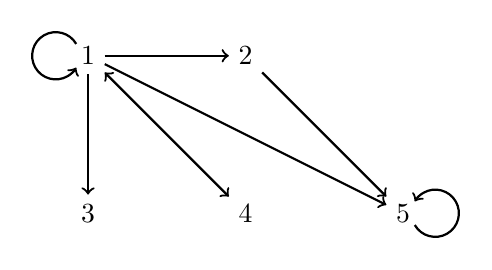
\begin{tikzpicture}
\node (atom1) at (0,2) {$1$};
\node (atom2) at (2,2) {$2$};
\node (atom4) at (0,0) {$3$};
\node (atom5) at (2,0) {$4$};
\node (atom6) at (4,0) {$5$};
\draw[->, thick] (atom1)+(-0.15,0.15) arc (-330:-30:.3); 
\draw[->, thick] (atom6)+(0.15,-0.15) arc (-150:150:.3); 
\draw[->, thick] (atom1) -- (atom2);
\draw[->, thick] (atom1) -- (atom4);
\draw[<->, thick] (atom1) -- (atom5);
\draw[->, thick] (atom1) -- (atom6);
\draw[->, thick] (atom2) -- (atom6);
\end{tikzpicture}
\end{bmlimage}\bmlDescription{The numbers 1, 2, 3, 4, and 5 are connected
by arrows. There are arrows from 1 to 2, 3, 4, 5, and to itself, from 2 to
5, from 5 to itself, and from 4 to 1. There is no arrow leaving 3.}
\end{center}
Determine whether each of the following sentences is true or false in that interpretation:
\begin{compactlist}
\item $\exists x\, \atom{R}{x,x}$
\item $\forall x\, \atom{R}{x,x}$
\item $\exists x \forall y\, \atom{R}{x,y}$
\item $\exists x \forall y\, \atom{R}{y,x}$
\item $\forall x \forall y \forall z ((\atom{R}{x,y} \eand \atom{R}{y,z}) \eif \atom{R}{x,z})$
\item $\forall x \forall y \forall z ((\atom{R}{x,y} \eand \atom{R}{x,z}) \eif \atom{R}{y,z})$
\item $\exists x \forall y\, \enot \atom{R}{x,y}$
\item $\forall x(\exists y\, \atom{R}{x,y} \eif \exists y\, \atom{R}{y,x})$
\item $\exists x \exists y (\enot x = y \eand \atom{R}{x,y} \eand \atom{R}{y,x})$
\item $\exists x \forall y(\atom{R}{x,y} \eiff x = y)$
\item $\exists x \forall y(\atom{R}{y,x} \eiff x = y)$
\item $\exists x \exists y(\enot x = y \eand \atom{R}{x,y} \eand \forall z(\atom{R}{z,x} \eiff y = z))$
\end{compactlist}


\chapter{Semantic concepts}

Defining truth in FOL was quite fiddly. But now that we are done, we can define various other central logical notions. These definitions will look very similar to those for TFL, from \S\ref{s:SemanticConcepts}. However, remember that they concern \emph{interpretations}, rather than valuations.

We will use the symbol `$\entails$' for FOL much as we did for TFL. So:
	$$\metav{A}_1, \metav{A}_2, \ldots, \metav{A}_n \entails\metav{C}$$
means that there is no interpretation in which all of $\metav{A}_1$, $\metav{A}_2$, \dots, $\metav{A}_n$ are true and in which \metav{C} is false. Derivatively,
	$$\entails\metav{A}$$
means that \metav{A} is true in every interpretation.

The other logical notions also have corresponding definitions in FOL:

\factoidbox{
An FOL sentence $\metav{A}$ is a \define{validity} \ifeff{} $\metav{A}$ is true in every interpretation; i.e.,  $\entails\metav{A}$.
\newglossaryentry{validity}
{
name=validity,
description={A \gls{sentence of FOL} that is true in every \gls{interpretation}}
}

\medskip\noindent$\metav{A}$ is a \define{contradiction} \ifeff{} $\metav{A}$ is false in every interpretation; i.e., $\entails\enot\metav{A}$.
\newglossaryentry{contradiction of FOL}
{
  name=contradiction (of FOL),
  text=contradiction,
description={A \gls{sentence of FOL} that is false in every \gls{interpretation}}
}
  
\medskip\noindent $\metav{A}_1, \metav{A}_2, \ldots, \metav{A}_n \therefore \metav{C}$ is \define{valid in FOL} \ifeff{} there is no interpretation in which all of the premises are true and the conclusion is false; i.e., $\metav{A}_1,\metav{A}_2,\ldots, \metav{A}_n \entails\metav{C}$. It is \define{invalid in FOL} otherwise.
\newglossaryentry{valid in FOL}
{
  name=validity of arguments (in FOL),
  text = valid,
description={A property held by arguments; an argument is valid if and only if no \gls{interpretation} makes all premises true and the conclusion false}
}

\medskip\noindent Two FOL sentences \metav{A} and \metav{B} are \define{equivalent} \ifeff{} they are true in exactly the same interpretations as each other; i.e., both $\metav{A}\entails\metav{B}$ and $\metav{B}\entails\metav{A}$.

\newglossaryentry{equivalent in FOL}
{
  name=equivalence (in FOL),
  text = equivalent,
description={A property held by pairs of \glspl{sentence of FOL} if and only if the sentences have the same truth value in every \gls{interpretation}}
}

\medskip\noindent The FOL sentences $\metav{A}_1$, $\metav{A}_2$, \dots, $\metav{A}_n$ are \define{jointly satisfiable} \ifeff{} some interpretation makes all of them true. They are \define{jointly unsatisfiable} \ifeff{} there is no such interpretation.
\newglossaryentry{satisfiable in FOL}
{
  name=satisfiability (in FOL),
  text=jointly satisfiable,
description={A property held by \glspl{sentence of FOL} if and only if some \gls{interpretation} makes all the sentences true}
}
}

\chapter{Using interpretations}
\label{sec.UsingModels}

\section{Validities and contradictions}
Suppose we want to show that `$\exists x\, \atom{A}{x,x} \eif \atom{B}{d}$' is \emph{not} a validity. This requires showing that the sentence is not true in every interpretation; i.e.,\ that it is false in some interpretation. If we can provide just one interpretation in which the sentence is false, then we will have shown that the sentence is not a validity.

In order for `$\exists x\,\atom{A}{x,x} \eif \atom{B}{d}$' to be false, the antecedent (`$\exists x\, \atom{A}{x,x}$') must be true, and the consequent (`$\atom{B}{d}$') must be false. To construct such an interpretation, we start by specifying a domain. Keeping the domain small makes it easier to specify what the predicates will be true of, so we will start with a domain that has just one member. For concreteness, let's say it is \emph{just} the city of Paris.
	\begin{ekey}
		\item[\text{domain}] Paris
	\end{ekey}
The name `$d$' must refer to something in the domain, so we have no option but:
	\begin{ekey}
		\item[d] Paris
	\end{ekey}
Recall that we want `$\exists x\, \atom{A}{x,x}$' to be true, so we want all members of the domain to be paired with themselves in the extension of `$A$'. We can just offer:
	\begin{ekey}
		\item[\atom{A}{x,y}] \gap{x} is identical with \gap{y}
	\end{ekey}
Now `$\atom{A}{d,d}$' is true, so it is surely true that `$\exists x\, \atom{A}{x,x}$'. Next, we want `$\atom{B}{d}$' to be false, so the referent of `$d$' must not be in the extension of `$B$'. We might simply offer:
	\begin{ekey}
		\item[\atom{B}{x}] \gap{x} is in Germany
	\end{ekey}
Now we have an interpretation where `$\exists x\, \atom{A}{x,x}$' is true, but where `$\atom{B}{d}$' is false. So there is an interpretation where `$\exists x\, \atom{A}{x,x} \eif \atom{B}{d}$' is false. So `$\exists x\, \atom{A}{x,x} \eif \atom{B}{d}$' is not a validity.

We can just as easily show that `$\exists x\atom{A}{x,x} \eif \atom{B}{d}$' is not a contradiction. We need only specify an interpretation in which `$\exists x\atom{A}{x,x} \eif \atom{B}{d}$' is true; i.e., an interpretation in which either `$\exists x\, \atom{A}{x,x}$' is false or `$\atom{B}{d}$' is true. Here is one:
	\begin{ekey}
		\item[\text{domain}] Paris
		\item[d] Paris
		\item[\atom{A}{x,y}] \gap{x} is identical with \gap{y}
		\item[\atom{B}{x}] \gap{x} is in France
	\end{ekey}
This shows that there is an interpretation where `$\exists x\atom{A}{x,x} \eif \atom{B}{d}$' is true. So `$\exists x\, \atom{A}{x,x} \eif \atom{B}{d}$' is not a contradiction.
	\factoidbox{
		To show that $\metav{A}$ is not a validity, it suffices to find an interpretation where $\metav{A}$ is false.
		
		\medskip\noindent To show that $\metav{A}$ is not a contradiction, it suffices to find an interpretation where $\metav{A}$ is true.
	}

\section{Logical equivalence}
Suppose we want to show that `$\forall x\, \atom{S}{x}$' and `$\exists x\, \atom{S}{x}$' are not logically equivalent. We need to construct an interpretation in which the two sentences have different truth values; we want one of them to be true and the other to be false. We start by specifying a domain. Again, we make the domain small so that we can specify extensions easily. In this case, we will need at least two objects. (If we chose a domain with only one member, the two sentences would end up with the same truth value. In order to see why, try constructing some partial interpretations with one-member domains.) For concreteness, let's take:
	\begin{ekey}
		\item[\text{domain}] Ornette Coleman, Miles Davis
	\end{ekey}
We can make `$\exists x\, \atom{S}{x}$' true by including something in the extension of `$S$', and we can make `$\forall x\, \atom{S}{x}$' false by leaving something out of the extension of `$S$'. For concreteness, let's say:
	\begin{ekey}
		\item[\atom{S}{x}] \gap{x} plays saxophone
	\end{ekey}
Now `$\exists x\, \atom{S}{x}$' is true, because `$\atom{S}{x}$' is true of Ornette Coleman. Slightly more precisely, extend our interpretation by allowing `$c$' to name Ornette Coleman.  `$\atom{S}{c}$' is true in this extended interpretation, so `$\exists x\, \atom{S}{x}$' was true in the original interpretation. Similarly, `$\forall x\, \atom{S}{x}$' is false, because `$\atom{S}{x}$' is false of Miles Davis. Slightly more precisely, extend our interpretation by allowing `$d$' to name Miles Davis, and `$\atom{S}{d}$' is false in this extended interpretation, so `$\forall x\, \atom{S}{x}$' was false in the original interpretation. We have provided a counter-interpretation to the claim that `$\forall x\, \atom{S}{x}$' and `$\exists x\, \atom{S}{x}$' are logically equivalent.
	\factoidbox{
		To show that $\metav{A}$ and $\metav{B}$ are not logically equivalent, it suffices to find an interpretation where one is true and the other is false.
	}

\section{Validity, entailment and satisfiability}
To test for validity, entailment, or satisfiability, we typically need to produce interpretations that determine the truth value of several sentences simultaneously.

Consider the following argument in FOL:
$$\exists x(\atom{G}{x} \eif \atom{G}{a}) \therefore \exists x\, \atom{G}{x} \eif \atom{G}{a}$$
To show that this is invalid, we must make the premise true and the conclusion false. The conclusion is a conditional, so to make it false, the antecedent must be true and the consequent must be false. Clearly, our domain must contain two objects. Let's try:
	\begin{ekey}
		\item[\text{domain}] Karl Marx, Ludwig von Mises
		\item[\atom{G}{x}] \gap{x} hated communism
		\item[a] Karl Marx
	\end{ekey}
Given that Marx wrote \emph{The Communist Manifesto}, `$\atom{G}{a}$' is plainly false in this interpretation. But von Mises famously hated communism, so `$\exists x\, \atom{G}{x}$' is true in this interpretation. Hence `$\exists x\, \atom{G}{x} \eif \atom{G}{a}$' is false, as required.

Does this interpretation make the premise true? Yes it does! Note that `$\atom{G}{a} \eif \atom{G}{a}$' is true. (Indeed, it is a validity.) But then certainly `$\exists x (\atom{G}{x} \eif \atom{G}{a})$' is true, so the premise is true, and the conclusion is false, in this interpretation. The argument is therefore invalid.

In passing, note that we have also shown that `$\exists x(\atom{G}{x} \eif \atom{G}{a})$' does \emph{not} entail `$\exists x\, \atom{G}{x} \eif \atom{G}{a}$', i.e., that $\exists x (\atom{G}{x} \eif \atom{G}{a}) \nentails \exists x \atom{G}{x} \eif \atom{G}{a}$. Equally, we have shown that the sentences `$\exists x (\atom{G}{x} \eif \atom{G}{a})$' and `$\enot (\exists x\, \atom{G}{x} \eif \atom{G}{a})$' are jointly satisfiable.

Let's consider a second example. Consider:
$$\forall x \exists y\, \atom{L}{x,y} \therefore \exists y \forall x\, \atom{L}{x,y}$$
Again, we want to show that this is invalid. To do this, we must make the premises true and the conclusion false. Here is a suggestion:
\begin{ekey}
	\item[\text{domain}] Canadian citizens currently in a domestic partnership with another Canadian citizen
	\item[\atom{L}{x,y}] \gap{x} is in a domestic partnership with \gap{y}
\end{ekey}
The premise is clearly true on this interpretation. Anyone in the domain is a Canadian citizen in a domestic partnership with some other Canadian citizen. That other citizen will also, then, be in the domain. So for everyone in the domain, there will be someone (else) in the domain with whom they are in a domestic partnership. Hence `$\forall x \exists y\, \atom{L}{x,y}$' is true. However, the conclusion is clearly false, for that would require that there is some single person who is in a domestic partnership with everyone in the domain, and there is no such person, so the argument is invalid. We observe immediately that the sentences `$\forall x \exists y\, \atom{L}{x,y}$' and `$\enot\exists y \forall x\, \atom{L}{x,y}$' are jointly satisfiable and that `$\forall x \exists y\, \atom{L}{x,y}$' does not entail `$\exists y \forall x\, \atom{L}{x,y}$'.

For our third example, we'll mix things up a bit. In \S\ref{s:Interpretations}, we described how we can present some interpretations using diagrams. For example:
\begin{center}
	\begin{bmlimage}
	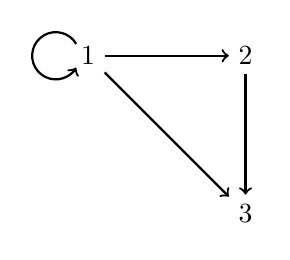
\begin{tikzpicture}
	\node (atom1) at (0,2) {1};
	\node (atom2) at (2,2) {2};
	\node (atom3) at (2,0) {3};
	\draw[->, thick] (atom1)--(atom2);
	\draw[->, thick] (atom1)--(atom3);
	\draw[->, thick] (atom1)+(-0.15,0.15) arc (-330:-30:.3); 
	\draw[->, thick] (atom2) -- (atom3);
\end{tikzpicture}
\end{bmlimage}\bmlDescription{The numbers 1, 2, and 3 are connected
by arrows. There are arrows from 1 to 2, 3, and to itself, and from 2 to
3. There is no arrow leaving 3.}
\end{center}
Using the conventions employed in \S\ref{s:Interpretations}, the domain of this interpretation is the first three positive whole numbers, and `$\atom{R}{x,y}$' is true of x and y just in case there is an arrow from x to y in our diagram. Here are some sentences that the interpretation makes true:
\begin{ebullet}
	\item `$\forall x \exists y\, \atom{R}{y,x}$' 
	\item `$\exists x \forall y\, \atom{R}{x,y}$' \hfill witness 1
	\item `$\exists x \forall y (\atom{R}{y,x} \eiff x = y)$' \hfill witness 1
	\item `$\exists x \exists y \exists z ((\enot y = z \eand \atom{R}{x,y}) \eand \atom{R}{z,x})$' \hfill witness 2
	\item `$\exists x \forall y\, \enot \atom{R}{x,y}$' \hfill witness 3
	\item `$\exists x (\exists y\, \atom{R}{y,x} \eand \enot \exists y\, \atom{R}{x,y})$' \hfill witness 3
\end{ebullet}
This immediately shows that all of the preceding six sentences are jointly satisfiable. We can use this observation to generate \emph{invalid} arguments, e.g.:
\begin{align*}
	\forall x \exists y\, \atom{R}{y,x}, \exists x \forall y\, \atom{R}{x,y}  &\therefore  \forall x \exists y\, \atom{R}{x,y}\\
	\exists x \forall y\, \atom{R}{x,y}, \exists x \forall y \enot \atom{R}{x,y} & \therefore \enot \exists x \exists y \exists z (\enot y = z \eand (\atom{R}{x,y} \eand \atom{R}{z,x}))
\end{align*}
and many more besides.

\factoidbox{
	If some interpretation makes all of $\metav{A}_1, \metav{A}_2, \ldots, \metav{A}_n$  true and $\metav{C}$ is false, then:
	\begin{compactlist}
		\item$\metav{A}_1, \metav{A}_2, \ldots, \metav{A}_n \therefore \metav{C}$ is \emph{invalid}; and
	\item $\metav{A}_1, \metav{A}_2, \ldots, \metav{A}_n \nentails \metav{C}$; and
	\item 
	And $\metav{A}_1, \metav{A}_2, \ldots, \metav{A}_n, \enot \metav{C}$ are jointly satisfiable.
\end{compactlist}}
An interpretation which refutes a claim---to logical truth, say, or to entailment---is called a \emph{counter-interpretation}, or a \emph{counter-model}.

We'll close this section, though, with a caution about the relationship between (in)validity and (non)entailment. Recall FOL's limitations: it is an extensional language; it ignores issues of vagueness; and it cannot handle cases of validity for `special reasons'. To take one illustration of these issues, consider this natural-language argument: 
\begin{earg}
	\item[] Every fox is cute.
	\item[\texttherefore] All vixens are cute.
\end{earg}
This is valid: necessarily every vixen is a fox, so it is impossible for the premise to be true and the conclusion false. Now, we might sensibly symbolize the argument as follows:
$$\forall x(\atom{F}{x} \eif \atom{C}{x}) \therefore \forall x(\atom{V}{x} \eif  \atom{C}{x})$$
However, it is easy to find counter-models which show that $\forall x(\atom{F}{x} \eif \atom{C}{x}) \nentails \forall x(\atom{V}{x} \eif  \atom{C}{x})$. (\emph{Exercise}: find one.) So, it would be \emph{wrong} to infer that the English argument is \emph{invalid}, just because there is a counter-model to the relevant \emph{FOL{}-entailment}.

The general moral is this. If you want to infer from the absence of an entailment in FOL to the invalidity of some English argument, then you need to argue that nothing important is lost in the way you have symbolized the English argument.

\practiceproblems

\solutions
\problempart
\label{pr.Contingent}
Show that each of the following is neither a validity nor a contradiction:
\begin{compactlist}
\item \leftsolutions\ $\atom{D}{a}  \eand \atom{D}{b}$
\item \leftsolutions\ $\exists x\, \atom{T}{x,h}$
\item \leftsolutions\ $\atom{P}{m}  \eand \enot\forall x\, \atom{P}{x}$
\item $\forall z \atom{J}{z} \eiff \exists y\, \atom{J}{y}$
\item $\forall x (\atom{W}{x,m,n} \eor \exists y\atom{L}{x,y})$
\item $\exists x (\atom{G}{x} \eif \forall y\, \atom{M}{y})$
\item $\exists x (x = h \eand x = i)$
\end{compactlist}

\solutions
\problempart
\label{pr.NotEquiv}
Show that the following pairs of sentences are not logically equivalent.
\begin{compactlist}
\item $\atom{J}{a} $,  $\atom{K}{a}$
\item $\exists x\, \atom{J}{x}$,  $\atom{J}{m}$
\item $\forall x\, \atom{R}{x,x}$, $\exists x\, \atom{R}{x,x}$
\item $\exists x\, \atom{P}{x} \eif \atom{Q}{c}$, $\exists x (\atom{P}{x} \eif \atom{Q}{c})$
\item $\forall x(\atom{P}{x} \eif \enot \atom{Q}{x})$, $\exists x(\atom{P}{x} \eand \enot \atom{Q}{x})$
\item $\exists x(\atom{P}{x} \eand \atom{Q}{x})$, $\exists x(\atom{P}{x} \eif \atom{Q}{x})$
\item $\forall x(\atom{P}{x}\eif \atom{Q}{x})$, $\forall x(\atom{P}{x} \eand \atom{Q}{x})$
\item $\forall x\exists y\, \atom{R}{x,y}$, $\exists x\forall y\, \atom{R}{x,y}$
\item $\forall x\exists y\, \atom{R}{x,y}$, $\forall x\exists y\, \atom{R}{y,x}$
\end{compactlist}



\problempart
Show that the following sentences are jointly satisfiable:
\begin{compactlist}
\item  $\atom{M}{a}, \enot \atom{N}{a}, \atom{P}{a}, \enot \atom{Q}{a}$
\item $\atom{L}{e,e}, \atom{L}{e,g}, \enot \atom{L}{g,e}, \enot \atom{L}{g,g}$
\item $\enot (\atom{M}{a} \eand \exists x\, \atom{A}{x}), \atom{M}{a} \eor \atom{F}{a}, \forall x(\atom{F}{x} \eif \atom{A}{x})$
\item $\atom{M}{a} \eor \atom{M}{b}, \atom{M}{a} \eif \forall x \enot \atom{M}{x}$
\item $\forall y\, \atom{G}{y}, \forall x (\atom{G}{x} \eif \atom{H}{x}), \exists y \enot \atom{I}{y}$
\item $\exists x(\atom{B}{x} \eor \atom{A}{x}), \forall x \enot \atom{C}{x}, \forall x\bigl[(\atom{A}{x} \eand \atom{B}{x}) \eif \atom{C}{x}\bigr]$
\item $\exists x\, \atom{X}{x}, \exists x\, \atom{Y}{x}, \forall x(\atom{X}{x} \eiff \enot \atom{Y}{x})$
\item $\forall x(\atom{P}{x} \eor \atom{Q}{x}), \exists x\enot(\atom{Q}{x} \eand \atom{P}{x})$
\item $\exists z(\atom{N}{z} \eand \atom{O}{z,z}), \forall x\forall y(\atom{O}{x,y} \eif \atom{O}{y,x})$
\item $\enot \exists x \forall y\, \atom{R}{x,y}, \forall x \exists y\, \atom{R}{x,y}$
\item $\enot \atom{R}{a,a}$, $\forall x (x=a \eor \atom{R}{x,a})$
\item $\forall x\forall y\forall z[(x=y \eor y=z )\eor x=z]$, $\exists x\exists y\ \enot x= y$
\item $\exists x\exists y((\atom{Z}{x} \eand \atom{Z}{y} )\eand x=y)$, $\enot \atom{Z}{d}$, $d=e$
\end{compactlist}

\problempart
Show that the following arguments are invalid:
\begin{compactlist}
\item $\forall x(\atom{A}{x} \eif \atom{B}{x}) \therefore \exists x\, \atom{B}{x}$
\item $\forall x(\atom{R}{x} \eif \atom{D}{x}), \forall x(\atom{R}{x} \eif \atom{F}{x}) \therefore \exists x(\atom{D}{x} \eand \atom{F}{x})$
\item $\exists x(\atom{P}{x}\eif \atom{Q}{x}) \therefore \exists x\, \atom{P}{x}$
\item $\atom{N}{a} \eand \atom{N}{b} \eand \atom{N}{c} \therefore \forall x\, \atom{N}{x}$
\item $\atom{R}{d,e}, \exists x\, \atom{R}{x,d} \therefore \atom{R}{e,d}$
\item $\exists x(\atom{E}{x} \eand \atom{F}{x}), \exists x\, \atom{F}{x} \eif \exists x\, \atom{G}{x} \therefore \exists x(\atom{E}{x} \eand \atom{G}{x})$
\item $\forall x\, \atom{O}{x,c}, \forall x\, \atom{O}{c,x} \therefore \forall x\, \atom{O}{x,x}$
\item $\exists x(\atom{J}{x} \eand \atom{K}{x}), \exists x \enot \atom{K}{x}, \exists x \enot \atom{J}{x} \therefore \exists x(\enot \atom{J}{x} \eand \enot \atom{K}{x})$
\item $\atom{L}{a,b} \eif \forall x\, \atom{L}{x,b}, \exists x\, \atom{L}{x,b} \therefore \atom{L}{b,b}$
\item $\forall x(\atom{D}{x} \eif \exists y\, \atom{T}{y,x}) \therefore \exists y \exists z\ \enot y= z$
\end{compactlist}

\chapter{Reasoning about interpretations}

\section{Validities and contradictions}
We can show that a sentence is \emph{not} a validity just by providing one carefully specified interpretation: an interpretation in which the sentence is false. To show that something \emph{is} a validity, on the other hand, it would not be enough to construct ten, one hundred, or even a thousand interpretations in which the sentence is true. A sentence is only a validity if it is true in \emph{every} interpretation, and there are infinitely many interpretations. We need to reason about all of them, and we cannot do this by dealing with them one by one!

Sometimes, we can reason about all interpretations fairly easily. For example, we can offer a relatively simple argument that `$\atom{R}{a,a}\eor\enot \atom{R}{a,a}$' is a validity:
	\begin{quote}
		\label{allmodels1}
		Any relevant interpretation will give `$\atom{R}{a,a}$' a truth value. If `$\atom{R}{a,a}$' is true in an interpretation, then `$\atom{R}{a,a} \eor \enot\atom{R}{a,a}$' is true in that interpretation. If `$\atom{R}{a,a}$' is false in an interpretation, then $\enot\atom{R}{a,a}$ is true, and so `$\atom{R}{a,a} \eor\enot \atom{R}{a,a}$' is true in that interpretation. These are the only alternatives. So `$\atom{R}{a,a} \eor\enot \atom{R}{a,a}$' is true in every interpretation. Therefore, it is a validity.
	\end{quote}
This argument is valid, of course, and its conclusion is true. However, it is not an argument in FOL. Rather, it is an argument in English \emph{about} FOL: it is an argument in the metalanguage.

Note another feature of the argument. Since the sentence in question contained no quantifiers, we did not need to think about how to interpret `$a$' and `$R$'; the point was just that, however we interpreted them, `$\atom{R}{a,a}$' would have some truth value or other. (We could ultimately have given the same argument concerning TFL sentences.)

Let's have another example. The sentence `$\forall x(\atom{R}{x,x}\eor\enot \atom{R}{x,x})$' should obviously be a validity. However, saying \emph{precisely} why is quite tricky. We cannot say that `$\atom{R}{x,x} \eor\enot \atom{R}{x,x}$' is true in every interpretation, since `$\atom{R}{x,x} \eor\enot \atom{R}{x,x}$' is not even a \emph{sentence} of FOL (remember that `$x$' is a variable, not a name). Instead, we should say something like this:
	\begin{quote}
		Consider some arbitrary interpretation. `$\forall x(\atom{R}{x,x}\eor \enot\atom{R}{x,x})$' is true in our interpretation \ifeff{} `$\atom{R}{x,x}\eor\enot\atom{R}{x,x}$' is satisfied by every object of its domain. Consider some arbitrary member of the domain, which, for convenience, we will call Fred. Either Fred satisfies `$\atom{R}{x,x}$' or it does not. If Fred satisfies `$\atom{R}{x,x}$', then Fred also satisfies `$\atom{R}{x,x} \eor \enot \atom{R}{x,x}$'. If Fred does not satisfy `$\atom{R}{x,x}$', it \emph{does} satisfy `$\enot\atom{R}{x,x}$' and so also `$\atom{R}{x,x} \eor\enot \atom{R}{x,x}$'.\footnote{We use here the fact that the truth conditions for connectives also apply to satisfaction: $a$ satisfies $\metav{A}(\metav{x}) \lor \metav{B}(\metav{x})$ \ifeff{} $a$ satisfies $\metav{A}(\metav{x})$ or $\metav{B}(\metav{x})$, etc.} So either way, Fred satisfies `$\atom{R}{x,x} \eor\enot \atom{R}{x,x}$'. Since there was nothing special about Fred---we might have chosen any object---we see that every object in the domain satisfies `$\atom{R}{x,x} \eor\enot \atom{R}{x,x}$'. So `$\forall x (\atom{R}{x,x} \eor\enot \atom{R}{x,x})$' is true in our interpretation. But we chose our interpretation arbitrarily, so `$\forall x (\atom{R}{x,x} \eor\enot \atom{R}{x,x})$' is true in every interpretation. It is therefore a validity.
	\end{quote}
This is quite long-winded, but, as things stand, there is no alternative. In order to show that a sentence is a validity, we must reason about \emph{all} interpretations.

\section{Other cases}
Similar points hold of other cases too. Thus, we must reason about all interpretations if we want to show:
	\begin{itemize}
		\item that a sentence is a contradiction (this requires that it is false in \emph{every} interpretation);
		\item that two sentences are logically equivalent (this requires that they have the same truth value in \emph{every} interpretation);
		\item that some sentences are jointly unsatisfiable (this requires that there is no interpretation in which all of those sentences are true together, i.e., that, in \emph{every} interpretation, at  least one of those sentences is false);
		\item that an argument is valid (this requires that the conclusion is true in \emph{every} interpretation where the premises are true);
		\item that some sentences entail another sentence.
	\end{itemize}
The problem is that, with the tools available to you so far, reasoning about all interpretations is a serious challenge! For a final example, here is a perfectly obvious entailment:
	$$\forall x(\atom{H}{x} \eand \atom{J}{x}) \entails \forall x\, \atom{H}{x}$$
After all, if everything is both $H$ and $J$, then everything is~$H$.
But we can only establish the entailment by considering what must be
true in every interpretation in which the premise $\forall
x(\atom{H}{x} \eand \atom{J}{x})$ is true. To show this, we would have
to reason as follows:
	\begin{quote}
		Consider an arbitrary interpretation in which `$\forall x(\atom{H}{x} \eand \atom{J}{x})$' is true. It follows that `$\atom{H}{x} \eand \atom{J}{x}$' is satisfied by every object in this interpretation. `$\atom{H}{x}$' will, then, also be satisfied by every object.\footnote{Here again we make use of the fact that any object that satisfies $\metav{A}(\metav{x}) \land \metav{B}(\metav{x})$ must satisfy both $\metav{A}(\metav{x})$ and $\metav{B}(\metav{x})$.} So it must be that `$\forall x\, \atom{H}{x}$' is true in the  interpretation. We've assumed nothing about the interpretation except that it was one in which `$\forall x(\atom{H}{x} \eand \atom{J}{x})$' is true. So any interpretation in which `$\forall x(\atom{H}{x} \eand \atom{J}{x})$' is true is one in which `$\forall x\, \atom{H}{x}$' is true.
\end{quote}
Even for a simple entailment like this one, the reasoning is somewhat complicated. For more complicated entailments, the reasoning can be extremely torturous.

The following table summarizes whether a single interpretation or counter-interpretation suffices, or whether we must reason about all interpretations.

\begin{center}\small
\begin{tabular}{l l l}
%\cline{2-3}
 & \textbf{Yes} & \textbf{No}\\
 \hline
%\cline{2-3}
validity? & all interpretations & one counter-interpretation\\
contradiction? &  all interpretations  & one counter-interpretation\\
equivalent? & all interpretations & one counter-interpretation\\
satisfiable? & one interpretation & all interpretations\\
valid? & all interpretations & one counter-interpretation\\
entailment? & all interpretations & one counter-interpretation\\
\end{tabular}
\end{center}
\label{table.ModelOrArgument}

You might want to compare this table with the table at the end of \S\ref{s:PartialTruthTable}. The key difference resides in the fact that TFL concerns truth tables, whereas FOL concerns interpretations. This difference is deeply important, since each truth-table only ever has finitely many lines, so that a complete truth table is a relatively tractable object. By contrast, there are infinitely many interpretations for any given sentence(s), so that reasoning about all interpretations can be a deeply tricky business.

\input{forallx-yyc-prooffol}
\input{forallx-yyc-ml}
%!TEX root = forallxyyc.tex
\part{Metatheory}
\label{ch.normalform}
\addtocontents{toc}{\protect\mbox{}\protect\hrulefill\par}

\chapter{Normal forms}\label{c:NormalForms}


\section{Disjunctive normal form}\label{s:DNFDefined}

Sometimes it is useful to consider sentences of a particularly simple form. For instance, we might consider sentences in which $\enot$ only attaches to atomic sentences, or those which are combinations of atomic sentences and negated atomic sentences using only $\eand$.  A relatively general but still simple form is that where a sentence is a disjunction of conjunctions of atomic or negated atomic sentences.  When such a sentence is constructed, we start with atomic sentences, then (perhaps) attach negations, then (perhaps) combine using $\eand$, and finally (perhaps) combine using~$\eor$. 

Let's say that a sentence is in \define{disjunctive normal form} \emph{iff} it meets all of the following conditions:
	\begin{earg}
		\item[(\textsc{dnf1})] No connectives occur in the sentence other than negations, conjunctions and disjunctions;
		\item[(\textsc{dnf2})] Every occurrence of negation has minimal scope (i.e.\ any `$\enot$' is immediately followed by an atomic sentence);
		\item[(\textsc{dnf3})] No disjunction occurs within the scope of any conjunction.
	\end{earg}
\newglossaryentry{disjunctive normal form}{
  name = disjunctive normal form (DNF),
  text = disjunctive normal form,
  description = {A sentence which is a disjunction of conjunctions of atomic sentences or negated atomic sentences}
}
So, here are are some sentences in disjunctive normal form:
\begin{align*}
  & A \\
  & (A \eand \lnot B \eand C)\\
  & (A \eand B) \eor (A \eand \enot B)\\
  & (A \eand B) \eor (A \eand  B \eand C \eand \enot D \eand \enot E)\\
  & A \eor (C \eand \enot P_{234} \eand P_{233} \eand Q) \eor \enot B
\end{align*}
Note that we have here broken one of the maxims of this book and \emph{temporarily} allowed ourselves to employ the relaxed bracketing-conventions that allow conjunctions and disjunctions to be of arbitrary length. These conventions make it easier to see when a sentence is in disjunctive normal form. We will continue to help ourselves to these relaxed conventions, without further comment.

To further illustrate the idea of disjunctive normal form, we will introduce some more notation. We write `$\pm\metav{A}$' to indicate that $\metav{A}$ is an atomic sentence which may or may not be prefaced with an occurrence of negation. Then a sentence in disjunctive normal form has the following shape:
	$$(\pm \metav{A}_1 \land \ldots \land \pm \metav{A}_i) \lor (\pm \metav{A}_{i+1} \land \ldots \land \pm\metav{A}_j) \lor \ldots \lor (\pm\metav{A}_{m+1} \land \ldots \land \pm \metav{A}_n)$$
We now know what it is for a sentence to be in disjunctive normal form. The result that we are aiming at is:
	\factoidbox{\label{thm:dnf}\textbf{Disjunctive Normal Form Theorem.} For any sentence, there is an equivalent sentence in disjunctive normal form.
	}
Henceforth, we will abbreviate `Disjunctive Normal Form' by `DNF'. 


\section{Proof of DNF theorem via truth tables}
\label{s:DNFTruthTable}

Our first proof of the DNF Theorem employs truth tables. We will first illustrate the technique for finding an equivalent sentence in DNF, and then turn this illustration into a rigorous proof. 

Let's suppose we have some sentence, $\metav{S}$, which contains three atomic sentences, `$A$', `$B$' and `$C$'. The very first thing to do is fill out a complete truth table for~$\metav{S}$. Maybe we end up with this:
\begin{center}
\begin{tabular}{c c c | c}
$A$ & $B$ & $C$ & $\metav{S}$\\
\hline
 T & T & T & T \\
 T & T & F & F \\
 T & F & T & T \\
 T & F & F & F \\
 F & T & T & F \\
 F & T & F & F \\
 F & F & T & T \\
 F & F & F & T
\end{tabular}
\end{center}
%Now, consider a sentence, whose only connectives are negations and conjunctions, where no connective occurs within the scope of any negation, e.g.:
%	$$A \eand \enot B \eand C$$
%This sentence is true when, and only when, `$A$' is true, `$B$' is false and `$C$' is true. Similarly, the sentence:
%	$$\enot A \eand \enot B \eand C$$
%this is true when, and only when, `$A$' is false, `$B$' is false and `$C$' is true. 
%
%A disjunction is true when, and only when, at least one of the disjuncts is true. So if we write down a disjunction of sentences of the above form, perhaps
%	$$(A \eand \enot B \eand C) \eor (\enot A \eand \enot B \eand C)$$
%then it will be true on exactly \emph{two} lines of the truth table which describes all possible valuations of `$A$', `$B$' and `$C$'. 
%
As it happens, $\metav{S}$ is true on four lines of its truth table, namely lines 1, 3, 7 and~8. Corresponding to each of those lines, we will write down four sentences, whose only connectives are negations and conjunctions, where every negation has minimal scope:
	\begin{earg}
		\item  `$A \eand B \eand C$'\hfill which is true on line 1 (and only then)
		\item `$A \eand \enot B \eand C$' \hfill which is true on line 3 (and only then)
		\item `$\enot A \eand \enot B \eand C$' \hfill which is true on line 7 (and only then)
		\item `$\enot A \eand \enot B \eand \enot C$' \hfill which is true on line 8 (and only then)
	\end{earg}
We now combine all of these conjunctions using~$\eor$, like so:
$$(A \eand B \eand C) \eor (A \eand \enot B \eand C) \eor (\enot A \eand \enot B \eand C) \eor (\enot A \eand \enot B \eand \enot C)$$\label{longDNF}
This gives us a sentence in DNF which is true on exactly those lines where one of the disjuncts is true, i.e.\ it is true on (and only on) lines 1, 3, 7, and 8. So this sentence has exactly the same truth table as $\metav{S}$. So we have a sentence in DNF that is logically equivalent to $\metav{S}$, which is exactly what we wanted!

Now, the strategy that we just adopted did not depend on the specifics of $\metav{S}$; it is perfectly general. Consequently, we can use it to obtain a simple proof of the DNF Theorem.

Pick any arbitrary sentence, $\metav{S}$, and let $\metav{A}_1, \ldots, \metav{A}_n$ be the atomic sentences that occur in $\metav{S}$. To obtain a sentence in DNF that is logically equivalent $\metav{S}$, we consider $\metav{S}$'s truth table. There are two cases to consider:
	\begin{enumerate}
		\item \emph{$\metav{S}$ is false on every line of its truth table.} Then, $\metav{S}$ is a contradiction. In that case, the contradiction $(\metav{A}_1 \eand \enot \metav{A}_1)$ is in DNF and logically equivalent to~$\metav{S}$. 
	
		\item \emph{$\metav{S}$ is true on at least one line of its truth table.}
		For each line $i$ of the truth table, let $\metav{B}_i$ be a conjunction of the form 
		$$(\pm\metav{A}_1 \land \ldots \land \pm\metav{A}_n)$$
		where the following rules determine whether or not to include a negation in front of each atomic sentence:
			\begin{align*}
				\metav{A}_m\text{ is a conjunct of }\metav{B}_i&\emph{ iff }\metav{A}_m\text{ is true on line }i\\
				\enot\metav{A}_m\text{ is a conjunct of }\metav{B}_i&\emph{ iff }\metav{A}_m\text{ is false on line }i
			\end{align*}
		Given these rules, $\metav{B_i}$ is true on (and only on) line $i$ of the truth table which considers all possible valuations of $\metav{A}_1, \ldots, \metav{A}_n$ (i.e.\ $\metav{S}$'s truth table). 
		
		Next, let $i_1$, $i_2$, \dots, $i_m$ be the numbers of the lines of the truth table where $\metav{S}$ is \emph{true}. Now let $\metav{D}$ be the sentence:
		$$\metav{B}_{i_1} \eor \metav{B}_{i_2} \eor \ldots \eor \metav{B}_{i_m}$$
		Since $\metav{S}$ is true on at least one line of its truth table, $\metav{D}$ is indeed well-defined; and in the limiting case where $\metav{S}$ is true on exactly one line of its truth table, $\metav{D}$ is just $\metav{B}_{i_1}$, for some $i_1$.
		
		By construction, $\metav{D}$ is in DNF. Moreover, by construction, for each line~$i$ of the truth table: $\metav{S}$ is true on line $i$ of the truth table \emph{iff} one of $\metav{D}$'s disjuncts (namely, $\metav{B_i}$) is true on, and only on, line $i$. Hence $\metav{S}$ and $\metav{D}$ have the same truth table, and so are logically equivalent.
	\end{enumerate}
	These two cases are exhaustive and, either way, we have a sentence in DNF that is logically equivalent to $\metav{S}$.

So we have proved the DNF Theorem. Before we say any more, though, we should immediately flag that we are hereby returning to the austere definition of a (TFL) sentence, according to which we can assume that any conjunction has exactly two conjuncts, and any disjunction has exactly two disjuncts.


\section{Conjunctive normal form}
\label{s:CNF}

So far in this chapter, we have discussed \emph{disjunctive} normal form. It may not come as a surprise to hear that there is also such a thing as \emph{conjunctive normal form} (CNF).

The definition of CNF is exactly analogous to the definition of DNF. So, a sentence is in CNF \emph{iff} it meets all of the following conditions:
	\begin{earg}
		\item[(\textsc{cnf1})] No connectives occur in the sentence other than negations, conjunctions and disjunctions;
		\item[(\textsc{cnf2})] Every occurrence of negation has minimal scope;
		\item[(\textsc{cnf3})] No conjunction occurs within the scope of any disjunction. 
	\end{earg}
\newglossaryentry{conjunctive normal form}{
  name = conjunctive normal form (DNF),
  text = conjunctive normal form,
  description = {A sentence which is a conjunction of disjunctions of atomic sentences or negated atomic sentences}
}
Generally, then, a sentence in CNF looks like this
	$$(\pm \metav{A}_1 \lor \ldots \lor \pm \metav{A}_i) \land (\pm \metav{A}_{i+1} \lor \ldots \lor \pm\metav{A}_j) \land \ldots \land (\pm\metav{A}_{m+1} \lor\ldots \lor \pm \metav{A}_n)$$
where each $\metav{A}_k$ is an atomic sentence.

We can now prove another normal form theorem:
	\factoidbox{\label{thm:cnf}\textbf{Conjunctive Normal Form Theorem.} For any sentence, there is an equivalent sentence in conjunctive normal form.}

        
	Given a TFL sentence, $\metav{S}$, we begin by writing down the complete truth table for $\metav{S}$.
	
	If $\metav{S}$ is \emph{true} on every line of the truth table, then $\metav{S}$ and $(\metav{A}_1 \eor \enot \metav{A}_1)$ are logically equivalent.
	
	If $\metav{S}$ is \emph{false} on at least one line of the truth table then, for every line on the truth table where $\metav{S}$ is false, write down a disjunction $(\pm\metav{A}_1 \eor \ldots \eor \pm\metav{A}_n)$ which is \emph{false} on (and only on) that line. Let $\metav{C}$ be the conjunction of all of these disjuncts; by construction, $\metav{C}$ is in CNF and $\metav{S}$ and $\metav{C}$ are logically equivalent.

\practiceproblems
\problempart
\label{pr.DNF}
Consider the following sentences:
	\begin{earg}
		\item $(A \eif \enot B)$
		\item $\enot (A \eiff B)$
		\item $(\enot A \eor \enot (A \eand B))$
		\item $(\enot (A \eif B ) \eand (A \eif C))$
		\item $(\enot (A \eor B) \eiff ((\enot C \eand \enot A) \eif \enot B))$
		\item $((\enot (A \eand \enot B) \eif C) \eand \enot (A \eand D))$
	\end{earg}
        For each sentence, find an equivalent sentence in DNF and one in CNF.

\chapter{Functional completeness}\label{c:FunctionalCompleteness}

Of our connectives, $\enot$ attaches to a single sentence, and the others all combine exactly two sentences. We may also introduce the idea of an $n$-place connective. For example, we could consider a three-place connective, `$\heartsuit$', and stipulate that it is to have the following characteristic truth table:
\begin{center}
\begin{tabular}{c c c | c}
$A$ & $B$ & $C$ & $\heartsuit(A,B,C)$\\
\hline
 T & T & T & F \\
 T & T & F & T \\
 T & F & T & T \\
 T & F & F & F \\
 F & T & T & F \\
 F & T & F & T \\
 F & F & T & F \\
 F & F & F & F
\end{tabular}
\end{center}
Probably this new connective would not correspond with any natural English expression (at least not in the way that `$\eand$' corresponds with `and'). But a question arises: if we wanted to employ a connective with this characteristic truth table, must we add a \emph{new} connective to TFL? Or can we get by with the connectives we \emph{already have} (as we can for the connective `neither\dots nor' for instance)?

Let us make this question more precise. Say that some connectives are \define{jointly functionally complete} \emph{iff}, for any possible truth table, there is a sentence containing only those connectives with that truth table.

\newglossaryentry{functionally complete}{
  name = {functional completeness},
  text = {functionally complete},
  description = {Property of a collection of connectives which holds iff every possible truth table is the truth table of a sentence involving only those connectives}}

The general point is, when we are armed with some jointly functionally complete connectives, no characteristic truth table lies beyond our grasp. And in fact, we are in luck.
	\factoidbox{\label{thm:ExpressiveAdequacy}\textbf{Functional Completeness Theorem.}
The connectives of TFL are jointly functionally complete. Indeed, the following pairs of connectives are jointly functionally complete:
\begin{earg}
\item\label{expressive:eor} `$\enot$' and `$\eor$'
\item\label{expressive:eand} `$\enot$' and `$\eand$'
\item\label{expressive:eif} `$\enot$' and `$\eif$'
\end{earg}}

Given any truth table, we can use the method of proving the DNF Theorem (or the CNF Theorem) via truth tables from chapter~\ref{c:NormalForms}, to write down a scheme which has the same truth table. For example, employing the truth table method for proving the DNF Theorem, we find that the following scheme has the same characteristic truth table as $\heartsuit(A,B,C)$, above:
		$$(A \eand B \eand \enot C) \eor (A \eand \enot B \eand C) \eor (\enot A \eand B \eand \enot C)$$			
It follows that the connectives of TFL are jointly functionally complete. We now prove each of the subsidiary results.
	
\emph{Subsidiary Result \ref{expressive:eor}: functional completeness of `$\enot$' and `$\eor$'.} Observe that the scheme that we generate, using the truth table method of proving the DNF Theorem, will only contain the connectives `$\enot$', `$\eand$' and `$\eor$'. So it suffices to show that there is an equivalent scheme which contains only `$\enot$' and `$\eor$'. To demonstrate this, we simply consider that
		\begin{align*}
		(\metav{A} \eand \metav{B}) & \text{\quad and \quad} \enot(\enot \metav{A} \eor\enot \metav{B})
		\end{align*}
		are logically equivalent.

\emph{Subsidiary Result \ref{expressive:eand}: functional completeness of `$\enot$' and `$\eand$'.} Exactly as in Subsidiary Result~\ref{expressive:eor}, making use of the fact that
		\begin{align*}
		(\metav{A} \eor \metav{B}) & \text{\quad and \quad}\enot(\enot \metav{A} \eand\enot \metav{B})
		\end{align*}
are logically equivalent.

\emph{Subsidiary Result \ref{expressive:eif}: functional completeness of `$\enot$' and `$\eif$'.} Exactly as in Subsidiary Result~\ref{expressive:eor}, making use of these equivalences instead:
		\begin{align*}
		(\metav{A} \eor \metav{B}) &\text{\quad and \quad} (\enot \metav{A} \eif \metav{B})\\
		(\metav{A} \eand \metav{B}) &\text{\quad and \quad} \enot(\metav{A} \eif \enot\metav{B})
		\end{align*}
Alternatively, we could simply rely upon one of the other two subsidiary results, and (repeatedly) invoke only one of these two equivalences.

In short, there is never any \emph{need} to add new connectives to TFL. Indeed, there is already some redundancy among the connectives we have: we could have made do with just two connectives, if we had been feeling really austere.

\section[Individually functionally complete connectives][Functionally complete connectives]{Individually functionally complete connectives}

In fact, some two-place connectives are \emph{individually} functionally complete. These connectives are not standardly included in TFL, since they are rather cumbersome to use. But their existence shows that, if we had wanted to, we could have defined a truth-functional language that was functionally complete, which contained only a single primitive connective.

The first such connective we will consider is `$\uparrow$', which has the following characteristic truth table. 
\begin{center}
\begin{tabular}{c c | c}
$\metav{A}$ & $\metav{B}$ & $\metav{A} \mathrel{\uparrow} \metav{B}$\\
\hline
 T & T & F \\
 T & F & T \\
 F & T & T  \\
 F & F & T
\end{tabular}
\end{center}
 This is often called `the Sheffer stroke', after Henry Sheffer, who used it to show how to reduce the number of logical connectives in Russell and Whitehead's \emph{Principia Mathematica}.\footnote{Sheffer, `A Set of Five Independent Postulates for Boolean Algebras, with application to logical constants,' (1913, \emph{Transactions of the American Mathematical Society} 14.4)} (In fact, Charles Sanders Peirce had anticipated Sheffer by about 30 years, but never published his results, and the Polish philosopher Erward Stamm published the same result two years before Sheffer.)\footnote{See Peirce, `A Boolian Algebra with One Constant', which dates to c.~1880, Peirce's \emph{Collected Papers}, 4.264--5, and Stamm, ``Beitrag zur Algebra der Logik,'' \emph{Monatshefte für Mathematik und Physik} 22 (1911): 137--49.} It is quite common, as well, to call it `nand', since its characteristic truth table is the negation of the truth table for `$\eand$'.
\factoidbox{\label{prop:upexpressive}`$\uparrow$' is functionally complete all by itself.}

The functional completeness Theorem tells us that `$\enot$' and `$\eor$' are jointly functionally complete. So it suffices to show that, given any scheme which contains only those two connectives, we can rewrite it as an equivalent scheme which contains only `$\uparrow$'. As in the proof of the subsidiary cases of the functional completeness Theorem, then, we simply apply the following equivalences:
		\begin{align*}
			\enot \metav{A} &\text{\quad and \quad} (\metav{A} \uparrow \metav{A})\\
			(\metav{A} \eor \metav{B}) & \text{\quad and \quad} ((\metav{A} \uparrow \metav{A}) \uparrow (\metav{B} \uparrow \metav{B}))
		\end{align*}
to the Subsidiary Result~\ref{expressive:eor}.

Similarly, we can consider the connective `$\downarrow$':
\begin{center}
\begin{tabular}{c c | c}
$\metav{A}$ & $\metav{B}$ & $\metav{A} \mathrel{\downarrow} \metav{B}$\\
\hline
 T & T & F \\
 T & F & F  \\
 F & T & F  \\
 F & F & T
\end{tabular}
\end{center}
This is sometimes called the `Peirce arrow' (Peirce himself called it `ampheck'). More often, though, it is called `nor', since its characteristic truth table is the negation of `$\eor$', that is, of `neither \dots{} nor \dots'.
	\factoidbox{
	`$\downarrow$' is functionally complete all by itself. }

As in the previous result for $\uparrow$, although invoking the equivalences:
		\begin{align*}
			\enot \metav{A} &\text{\quad and \quad} (\metav{A} \downarrow \metav{A})\\
			(\metav{A} \eand \metav{B}) & \text{\quad and \quad} ((\metav{A} \downarrow \metav{A}) \downarrow (\metav{B} \downarrow \metav{B}))
		\end{align*}
and Subsidiary Result~\ref{expressive:eand}.


\section{Failures of functional completeness}

In fact, the \emph{only} two-place connectives which are individually functionally complete are `$\uparrow$' and `$\downarrow$'. But how would we show this? More generally, how can we show that some connectives are \emph{not} jointly functionally complete? 
 
The obvious thing to do is to try to find some truth table which we \emph{cannot} express, using just the given connectives. But there is a bit of an art to this.

To make this concrete, let's consider the question of whether `$\eor$' is functionally complete all by itself. After a little reflection, it should be clear that it is not. In particular, it should be clear that any scheme which only contains disjunctions cannot have the same truth table as negation, i.e.:
				\begin{center}
				\begin{tabular}{c | c}
				$\metav{A}$ & $\enot \metav{A}$\\
				\hline
				 T & F \\
				 F & T
				\end{tabular}
				\end{center}
The intuitive reason, why this should be so, is simple: the top line of the desired truth table needs to have the value False; but the top line of any truth table for a scheme which \emph{only} contains $\eor$ will always be True. The same is true for $\eand$, $\eif$, and $\eiff$.
 	\factoidbox{
		`$\eor$', `$\eand$', `$\eif$', and `$\eiff$' are not functionally complete by themselves.}

In fact, the following is true:
        
\factoidbox{The \emph{only} two-place connectives that are functionally complete by themselves are `$\uparrow$' and `$\downarrow$'. }

This is of course harder to prove than for the primitive connectives. For instance, the ``exclusive or'' connective does not have a T in the first line of its characteristic truth table, and so the method used above no longer suffices to show that it cannot express all truth tables.  It is also harder to show that, e.g., `$\eiff$' and `$\enot$' \emph{together} are not functionally complete.

\chapter{Proving equivalences}\label{ch:equivalences}

\section{Substitutability of equivalents}

Recall from \S\ref{sec:equivalent} that $\metav{P}$ and $\metav{Q}$ are equivalent (in TFL) iff, for every valuation, their truth values agree.  We have seen many examples of this and used both truth tables and natural dedcution proofs to establish such equivalences.  In chapter~\ref{c:NormalForms} we've even proved that ever sentence of TFL is equivalent to one in conjunctive and one in disjunctive normal form.  If $\metav{P}$ and $\metav{Q}$ are equivalent, they always have the same truth value, either one entails the other, and from either one you can prove the other.

Equivalent sentences are not the same, of course: the sentences $\enot\enot A$ and~$A$ may always have the same truth value, but the first starts with the `$\enot$' symbol while the second doesn't.  But you may wonder if it's always true that we can replace one of a pair of equivalent sentences by the other, and the results will be equivalent, too.  For instance, consider $\enot\enot A \eif B$ and $A \eif B$.  The second results from the first by replacing `$\enot\enot A$' by~`$A$'.  And these two sentences are also equivalent.

This is a general fact, and it is not hard to see why it is true.  In any valuation, we compute the truth value of a sentence ``from the inside out.'' So when it comes to determining the truth value of `$\enot\enot A \eif B$', we first compute the truth value of `$\enot\enot A$', and the truth value of the overall sentence then just depends on that truth value (true or false, as the case may be) and the rest of the sentence (the truth value of~`$B$' and the truth table for~`$\eif$'). But since `$\enot\enot A$' are equivalent, they always have the same truth value in a given valuation---hence, replacing `$\enot\enot A$' by~`$A$' cannot change the truth value of the overall sentence.  The same of course is true for any other sentence equivalent to `$\enot\enot A$', say, `$A \eand (A \eor A)$'.

To state the result in general, let's use the notation $\metav{R}(\metav{P})$ to mean a sentence which contains the sentence $\metav{P}$ as a part. Then by $\metav{R}(\metav{Q})$ we mean the result of replacing the occurrence of $\metav{P}$ by the sentence~$\metav{Q}$.  For instance, if $\metav{P}$ is the sentence letter~`$A$', $\metav{Q}$ is the sentence~`$\enot\enot A$', and $\metav{R}(\metav{P})$ is `$A \eif B$', then $\metav{R}(\metav{Q})$ is `$\enot\enot A \eif B$'.

\factoidbox{If $\metav{P}$ and $\metav{Q}$ are equivalent, then so are $\metav{R}(\metav{P})$ and $\metav{R}(\metav{P})$.}

It follows from this fact that any sentence of the form $\metav{R}(\metav{P}) \eiff \metav{R}(\metav{P})$, where $\metav{P}$ and $\metav{Q}$ are equivalent, is a tautology. However, the proofs in natural deduction will be wildly different for different~$\metav{R}$. (As an exercise, give proofs that show that 
\begin{align*}
	& \vdash (\enot\enot P \eif Q) \eiff (P \eif Q)  \text{ and}\\
	& \vdash (\enot\enot P \eand Q) \eiff (P \eand Q)
\end{align*}
and compare the two.)

Here is another fact: if two sentences $\metav{P}$ and~$\metav{Q}$ are equivalent, and you replace some sentence letter in both $\metav{P}$ and $\metav{Q}$ by the same sentence~$\metav{R}$, the results are also equivalent.  For instance, if you replace `$A$' in both `$A \land B$' and `$B \land A$' by, say, `$\enot C$', you get `$\enot C \land B$' and `$B \land \enot C$', and those are equivalent. We can record this, too:

\factoidbox{Equivalence is preserved under replacement of sentence letters, i.e., if $\metav{P}(A)$ and $\metav{Q}(A)$ both contain the sentence letter~`$A$' and are equivalent, then the sentences $\metav{P}(\metav{R})$ and $\metav{Q}(\metav{R})$ (resulting by replacing `$A$' by $\metav{R}$ in both) are also equivalent.}

This means that once we have shown that two sentence are equivalent (e.g., `$\enot\enot A$' and `$A$', or `$A \land B$' and `$B \land A$') we know that all their common ``instances'' are also equivalent.  Note that we do not immediately get this from a truth table or a natural deduction proof. E.g., a truth table that shows that `$\enot\enot A$' and~`$A$' are equivalent does \emph{not} also show that `$\enot\enot(B \eif C)$' and `$B \eif C$' are equivalent: the former needs just 2 lines, the latter~4.

\section{Chains of equivalences}

When you want to verify that two sentences are equivalent, you can of course do a truth table, or look for a formal proof.  But there is a simpler method, based on the principle of substitutability of equivalents we just discussed: Armed with a small catalog of simple equivalences, replace parts of your first sentence by equivalent parts, and repeat until you reach your second sentence.

This method of showing sentences equivalent is underwritten by the two facts from the previous section. The first fact tells us that \emph{if}, say, $\enot\enot \metav{P}$ and $\metav{P}$ are equivalent (for any sentence~$\metav{P}$), then replacing $\enot\enot\metav{P}$ in a sentence by~$\metav{P}$ results in an equivalent sentence. The second fact tells us \emph{that} $\enot\enot \metav{P}$ and~$\metav{P}$ are always equivalent, for any sentence~$\metav{P}$. (A simple truth table shows that `$\enot\enot A$' and~`$A$' are equivalent.) By the second fact we know that whenever we replace `$A$' in both `$\enot\enot A$' and~`$A$' by some sentence~$\metav{P}$, we get equivalent results. In other words, from the fact that `$\enot\enot A$' and~`$A$' are equivalent and the second fact, we can conclude that, for any sentence~$\metav{P}$, $\enot\enot \metav{P}$ and~$\metav{P}$ are equivalent.

Let's give an example. By De Morgan's Laws, the following pairs of sentences are equivalent:
\begin{align*}
	\enot (A \eand B) & \text{ and } (\enot A \eor \enot B)\\
	\enot (A \eor B) & \text{ and } (\enot A \eand \enot B)
\end{align*}
This can be verified by constructing two truth tables, or four natural deduction proofs that show:
\begin{align*}
	\enot (A \eand B) & \vdash (\enot A \eor \enot B)\\
	(\enot A \eor \enot B) & \vdash \enot (A \eand B)\\
	\enot (A \eor B) & \vdash (\enot A \eand \enot B)\\
	(\enot A \eand \enot B) & \vdash \enot (A \eor B)
\end{align*}

By the second fact, \emph{any} pairs of sentences of the following forms are equivalent:
\begin{align*}
	\enot (\metav{P} \eand \metav{Q}) & \text{ and } (\enot \metav{P} \eor \enot \metav{Q})\\
	\enot (\metav{P} \eor \metav{Q}) & \text{ and } (\enot \metav{P} \eand \enot \metav{Q})
\end{align*}
Now consider the sentence `$\enot(R \eor (S \eand T))$'. We will find an equivalent sentence in which all `$\enot$' signs attach directly to sentence letters. In the first step, we consider this as a sentence of the form $\enot(\metav{P} \eor \metav{Q})$---then $\metav{P}$ is the sentence~`$R$' and $\metav{Q}$ is `$(S \eand T)$'. Since $\enot(\metav{P} \eor \metav{Q})$ is equivalent to $(\enot \metav{P} \eand \enot \metav{Q})$ (by the second of De Morgan's Laws) we can replace the entire sentence by $(\enot \metav{P} \eand \enot \metav{Q})$. In this case (where $\metav{P}$ is~`$R$' and $\metav{Q}$ is~`$(S \eand T)$') we obtain `$(\enot R \eand \enot (S \eand T))$'. This new sentence contains as a part the sentence `$\enot (S \eand T)$'. It is of the form $\enot(\metav{P} \eand \metav{Q})$, except now $\metav{P}$ is the sentence letter~`$S$' and $\metav{Q}$ is~`$T$'. By De Morgan's Law (the first one this time), this is equivalent to $(\enot\metav{P} \eor \enot\metav{Q})$, or in this specific case, to `$(\enot S \eor \enot T)$'. So we can replace the part `$\enot (S \eand T)$' by `$(\enot S \eor \enot T)$'. This now results in the sentence `$(\enot R \eand (\enot S \eor \enot T))$', in which the `$\enot$' symbols all attach directly to sentence letters. We've ``pushed'' the negations inwards as far as possible.  We can record such a chain of equivalences by listing the individual steps, and recording, just as we do in natural deduction, which basic equivalence we use in each case:
\begin{align*}
	& \fbox{\enot(\fbox{$R$} \eor \fbox{$(S \eand T)$})} \\
	& \fbox{(\enot(\fbox{$R$} \eand \enot\fbox{$(S \eand T)$})} && \text{DeM}\\
	& (\enot(R \eand \fbox{$\enot(\fbox{$S$} \eand \fbox{$T$})$}) \\
	& (\enot(R \eand \fbox{$(\enot \fbox{$S$} \eor \enot \fbox{$T$})$}) && \text{DeM}
\end{align*}
We've highlighted the sentence replaced, and those matching the $\metav{P}$ and~$\metav{Q}$ in De Morgan's Laws for clarity, but this is not necessary, and we won't keep doing it.

In table~\ref{tab:equivalences} we've given a list of basic equivalences you can use for such chains of equivalences. The labels abbreviate the customary name for the respective logical laws: double negation (DN), De Morgan (DeM), commutativity (Comm), distributivity (Dist), associativity (Assoc), idempotence (Id), and absorption (Abs).

\begin{table}
	\begin{align*}
\lnot\lnot \metav{P} & \Leftrightarrow \metav{P} && \text{(DN)}\\[2ex]
(\metav{P} \eif \metav{Q}) & \Leftrightarrow (\lnot \metav{P} \lor \metav{Q})
&& \text{(Cond)}\\
\lnot(\metav{P} \eif \metav{Q}) & \Leftrightarrow (\metav{P} \land \lnot\metav{Q}) \\[2ex]
(\metav{P} \eiff \metav{Q}) & \Leftrightarrow ((\metav{P} \eif \metav{Q}) \land  (\metav{Q} \eif \metav{P}))
&& \text{(Bicond)}\\[2ex]
\lnot(\metav{P} \land \metav{Q}) & \Leftrightarrow (\lnot\metav{P} \lor \lnot\metav{Q})
&& \text{(DeM)}\\
\lnot(\metav{P} \lor \metav{Q}) & \Leftrightarrow (\lnot\metav{P} \land \lnot\metav{Q}) \\[2ex]
(\metav{P} \lor \metav{Q}) & \Leftrightarrow (\metav{Q} \lor \metav{P}) & &\text{(Comm)}\\
(\metav{P} \land \metav{Q}) & \Leftrightarrow (\metav{Q} \land \metav{P})\\[2ex]
(\metav{P} \land (\metav{Q} \lor \metav{R})) & \Leftrightarrow ((\metav{P} \land \metav{Q}) \lor (\metav{P} \land \metav{R}))
&& \text{(Dist)}\\
(\metav{P} \lor (\metav{Q} \land \metav{R})) & \Leftrightarrow ((\metav{P} \lor \metav{Q}) \land (\metav{P} \lor \metav{R}))\\
(\metav{P} \lor (\metav{Q} \lor \metav{R})) & \Leftrightarrow ((\metav{P} \lor \metav{Q}) \lor \metav{R}) & &\text{(Assoc)}\\
(\metav{P} \land (\metav{Q} \land \metav{R})) & \Leftrightarrow ((\metav{P} \land \metav{Q}) \land \metav{R})\\[2ex]
(\metav{P} \lor \metav{P}) & \Leftrightarrow \metav{P} && \text{(Id)}\\
(\metav{P} \land \metav{P}) & \Leftrightarrow \metav{P}\\[2ex]
(\metav{P} \land (\metav{P} \lor \metav{Q})) & \Leftrightarrow \metav{P}&& \text{(Abs)}\\
(\metav{P} \lor (\metav{P} \land \metav{Q})) & \Leftrightarrow \metav{P}\\[2ex]
(\metav{P} \land (\metav{Q} \lor \lnot\metav{Q})) & \Leftrightarrow \metav{P}  && \text{(Simp)}\\
(\metav{P} \lor (\metav{Q} \land \lnot\metav{Q})) & \Leftrightarrow \metav{P}\\[2ex]
(\metav{P} \lor (\metav{Q} \lor \lnot\metav{Q})) & \Leftrightarrow (\metav{Q} \lor \lnot\metav{Q}) \\
(\metav{P} \land (\metav{Q} \land \lnot\metav{Q})) & \Leftrightarrow (\metav{Q} \land \lnot\metav{Q})
\end{align*}
\caption{Basic equivalences}
\label{tab:equivalences}
\end{table}

\section{Finding equivalent normal forms}

In chapter~\ref{c:NormalForms} we showed that every sentence of TFL is equivalent to one in disjunctive normal form (DNF) and to one in conjunctive normal form (CNF).  We did this by giving a method to construct a sentences in DNF or CNF equivalent to the original sentence by first constructing a truth table, and then ``reading off'' a sentence in DNF or CNF from the truth table.  This method has two drawbacks. The first one is that the resulting sentences in DNF or CNF are not always the shortest ones.  The second one is that the method itself becomes hard to apply when the sentence you start with contains more than a handful of sentence letters (since the truth table for a sentence with $n$ sentence letters has $2^n$ lines).

We can use chains of equivalences as an alternative method: To find a sentence in~DNF, we can successively apply basic equivalences until we have found an equivalent sentence that is in~DNF. Recall the conditions a sentence in DNF must satisfy:
\begin{earg}
	\item[(\textsc{dnf1})] No connectives occur in the sentence other than negations, conjunctions and disjunctions;
	\item[(\textsc{dnf2})] Every occurrence of negation has minimal scope (i.e., any `$\enot$' is immediately followed by an atomic sentence);
	\item[(\textsc{dnf3})] No disjunction occurs within the scope of any conjunction.
\end{earg}
Condition (\textsc{dnf1}) says that we must remove all `$\eif$' and~`$\eiff$' symbols from a sentence.  This is what the basic equivalences (Cond) and (Bicond) are good for.  For instance, suppose we start with the sentence
\begin{align*}
	& \enot(A \eand \enot C) \land (\enot A\eif \enot B).
\intertext{We can get rid of the `$\eif$' by using (Cond). In this case $\metav{P}$ is `$\enot A$' and $\metav{Q}$ is `$\enot{B}$'. We get:}
& \enot(A \eand \enot C) \land (\enot\enot A \eor \enot B) && \text{Cond}
\intertext{The double negation can be removed, since `$\enot\enot A$' is equivalent to~`$A$':}
& \enot(A \eand \enot C) \land (A \eor \enot B) && \text{DN}
\intertext{Now condition (\textsc{dnf1}) is satisfied: our sentence contains only `$\enot$', `$\eand$', and `$\eor$'. Condition (\textsc{dnf2}) says that we must find a way to have all `$\enot$'s apply immediately to sentence letters. But in the first conjunct it doesn't.  To ensure (\textsc{dnf2}) is satisfied, we use De Morgan's Laws and the double negation (DN) law as many times as needed.}
& (\enot A \eor \enot\enot C) \land (A \eor \enot B) && \text{DeM}\\
& (\enot A \eor C) \land (A \eor \enot B) && \text{DN}
\intertext{The resulting sentence is now in CNF---it is a conjunction of disjunctions of sentence letters and negated sentence letters. But we want a sentence in DNF, i.e., a sentence in which (\textsc{dnf3}) is satisfied: no `$\eor$' occurs in the scope of an~`$\eand$'.  We use the distributive laws (Dist) to ensure this. The last sentence is of the form $\metav{P} \land (\metav{Q} \lor \metav{R})$, where $\metav{P}$ is `$(\enot A \eor C)$', $\metav{Q}$ is `$A$', and $\metav{R}$ is `$\enot B$'. By applying (Dist) once we get:}
& ((\enot A \eor C) \eand A)) \eor ((\enot A \eor C) \eand \enot B) && \text{Dist}
\intertext{This looks worse, but if we keep going, it's going to look better! The two disjuncts almost look like we can apply (Dist) again, except the `$\eor$' is on the wrong side. This is what commutativity (Comm) is good for. let's apply it to `$(\enot A \eor C) \eand A$':}
& (A \eand (\enot A \eor C)) \eor ((\enot A \eor C) \eand \enot B) && \text{Comm}
\intertext{We can apply (Dist) again to the resulting part, `$A \eand (\enot A \eor C)$':}
& ((A \eand \enot A) \eor (A \eand C)) \eor ((\enot A \eor C) \eand \enot B) && \text{Dist}
\intertext{Now in the left half, no `$\eor$' is in the scope of an `$\eand$'. Let's apply the same principles to the right half:}
& ((A \eand \enot A) \eor (A \eand C)) \eor (\enot B \eand (\enot A \eor C)) && \text{Comm}\\
& ((A \eand \enot A) \eor (A \eand C)) \eor ((\enot B \eand \enot A) \eor (\enot B \eand C)) && \text{Dist}
\intertext{Our sentence is now in DNF! But we can simplify it a bit: `$(A \eand \enot A)$' is a contradiction in TFL, i.e., it is always false. And if you combine something that's always false using `$\eor$' with a sentence~$\metav{P}$, you get something equivalent to just~$\metav{P}$.  This is the second of the simplification (Simp) rules.}
& ((A \eand C) \eor (A \eand \enot A)) \eor ((\enot B \eand \enot A) \eor (\enot B \eand C)) && \text{Comm}\\
& (A \eand C) \eor ((\enot B \eand \enot A) \eor (\enot B \eand C)) && \text{Simp}
\end{align*}
The final result is still in DNF, but a bit simpler still.  It is also much simpler than the DNF we would have obtained by the method of chapter~\ref{c:NormalForms}. In fact, the sentence we started with could have been the $\metav{S}$ of \S\ref{s:DNFTruthTable}---it has exactly the truth table used as an example there. The DNF we found there (on p.~\pageref{longDNF}), was (with all necessary brackets):
$$((((A \eand B) \eand C) \eor ((A \eand \enot B) \eand C)) \eor ((\enot A \eand \enot B) \eand C)) \eor ((\enot A \eand \enot B) \eand \enot C).$$

\practiceproblems
\problempart
\label{pr.DNF2}
Consider the following sentences:
\begin{earg}
	\item $(A \eif \enot B)$
	\item $\enot (A \eiff B)$
	\item $(\enot A \eor \enot (A \eand B))$
	\item $(\enot (A \eif B ) \eand (A \eif C))$
	\item $(\enot (A \eor B) \eiff ((\enot C \eand \enot A) \eif \enot B))$
	\item $((\enot (A \eand \enot B) \eif C) \eand \enot (A \eand D))$
\end{earg}
For each sentence, find an equivalent sentence in DNF and one in CNF by giving a chain of equivalences. Use (Id), (Abs), and (Simp) to simplify your sentences as much as possible.

\chapter{Soundness}\label{ch:Soundness}

In this chapter we relate TFL's semantics to its natural deduction \emph{proof system} (as defined in Part~\ref{ch.NDTFL}). We will prove that the formal proof system is safe: you can only prove sentences from premises from which they actually follow.
Intuitively, a formal proof system is sound iff it does not allow you to prove any invalid arguments. This is obviously a highly desirable property. It tells us that our proof system will never lead us astray. Indeed, if our proof system were not sound, then we would not be able to trust our proofs. The aim of this chapter is to prove that our proof system is sound.

Let's make the idea more precise. We'll abbreviate a list of sentences using the greek letter $\Gamma$ (`gamma'). A formal proof system is \define{sound} (relative to a given semantics) \emph{iff}, whenever there is a formal proof of $\metav{C}$ from assumptions among $\Gamma$, then $\Gamma$ genuinely entails $\metav{C}$ (given that semantics). Otherwise put, to prove that TFL's proof system is sound, we need to prove the following

\begin{factoidboxe}\textbf{Soundness Theorem.} For any sentences $\Gamma$ and $\metav{C}$: if $\Gamma\proves\metav{C}$, then $\Gamma \entails\metav{C}$
\end{factoidboxe}

To prove this, we will check each of the rules of TFL's proof system individually. We want to show that no application of those rules ever leads us astray. Since a proof just involves repeated application of those rules, this will show that no proof ever leads us astray. Or at least, that is the general idea.

To begin with, we must make the idea of `leading us astray' more precise. Say that a line of a proof is \define{shiny} iff the assumptions on which that line depends entail the sentence on that line.\footnote{The word `shiny' is not standard among logicians.} To illustrate the idea, consider the following:
	\begin{fitchproof}
		\hypo{fgh}{F\eif(G\eand H)}
		\open
			\hypo{f}{F}
			\have{gh}{G \eand H}\ce{fgh,f}
			\have{g}{G}\ae{gh}
		\close
		\have{fg}{F \eif G}\ci{f-g}
	\end{fitchproof}\noindent\noindent
Line $1$ is shiny iff $F \eif (G \eand H) \entails F \eif (G \eand H)$. You should be easily convinced that line $1$ is, indeed, shiny! Similarly, line $4$ is shiny iff $F \eif (G \eand H), F \entails G$. Again, it is easy to check that line $4$ is shiny. As is every line in this TFL-proof. We want to show that this is no coincidence. That is, we want to prove:
	\begin{factoidboxe}\textbf{Shininess Lemma.}
		Every line of every TFL-proof is shiny.
	\end{factoidboxe}\noindent
Then we will know that we have never gone astray, on any line of a proof. Indeed, given the Shininess Lemma, it will be easy to prove the Soundness Theorem:

\emph{Proof.} Suppose $\Gamma \proves \metav{C}$. Then there is a TFL-proof, with $\metav{C}$ appearing on its last line, whose only undischarged assumptions are among $\Gamma$. The Shininess Lemma tells us that every line on every TFL-proof is shiny. So this last line is shiny, i.e.\ $\Gamma \entails \metav{C}$. QED

It remains to prove the Shininess Lemma. 

To do this, we observe that every line of any TFL-proof is obtained by applying some rule. So what we want to show is that no application of a rule of TFL's proof system will lead us astray. More precisely, say that a rule of inference is \define{rule-sound} \emph{iff} for all TFL-proofs, if we obtain a line on a TFL-proof by applying that rule, and every earlier line in the TFL-proof is shiny, then our new line is also shiny. What we need to show is that \emph{every} rule in TFL's proof system is rule-sound. 

We will do this in the next section. But having demonstrated the rule-soundness of every rule, the Shininess Lemma will follow immediately:

\emph{Proof.} Fix any line, line $n$, on any TFL-proof. The sentence written on line $n$ must be obtained using a formal inference rule which is rule-sound. This is to say that, if every earlier line is shiny, then line $n$ itself is shiny. Hence, by strong induction on the length of TFL-proofs, every line of every TFL-proof is shiny. QED

Note that this proof appeals to a principle of strong induction on the length of TFL-proofs. This is the first time we have seen that principle, and you should pause to confirm that it is, indeed, justified.

It remains to show that every rule is rule-sound. This is not difficult, but it is time-consuming, since we need to check each rule individually, and TFL's proof system has plenty of rules! To speed up the process marginally, we will introduce a convenient abbreviation: `$\Delta_i$' (`delta') will abbreviate the assumptions (if any) on which line $i$ depends in our TFL-proof (context will indicate which TFL-proof we have in mind).

\begin{factoidboxe}Introducing an assumption is rule-sound.
\end{factoidboxe}

If $\metav{A}$ is introduced as an assumption on line $n$, then $\metav{A}$ is among $\Delta_n$, and so $\Delta_n \entails \metav{A}$.

\begin{factoidboxe}$\eand$I is rule-sound.
\end{factoidboxe}

\emph{Proof.} Consider any application of $\eand$I in any TFL-proof, i.e., something like:
\begin{fitchproof}
	\have[i]{a}{\metav{A}}
	\have[j]{b}{\metav{B}}
	\have[n]{c}{\metav{A}\eand\metav{B}} \ai{a, b}
\end{fitchproof}\noindent
To show that $\eand$I is rule-sound, we assume that every line before line $n$ is shiny; and we aim to show that line $n$ is shiny, i.e.\ that $\Delta_n \entails \metav{A} \eand \metav{B}$. 

So, let $v$ be any valuation that makes all of $\Delta_{n}$ true. 

We first show that $v$ makes $\metav{A}$ true. To prove this, note that all of $\Delta_i$ are among $\Delta_{n}$. By hypothesis, line $i$ is shiny. So any valuation that makes all of $\Delta_i$ true makes $\metav{A}$ true. Since $v$ makes all of $\Delta_i$ true, it makes $\metav{A}$ true too.

We can similarly see that $v$ makes $\metav{B}$ true. 

So $v$ makes $\metav{A}$ true and $v$ makes $\metav{B}$ true. Consequently, $v$ makes $\metav{A}\eand\metav{B}$ true. So any valuation that makes all of the sentences among $\Delta_{n}$ true also makes $\metav{A} \eand \metav{B}$ true. That is: line $n$ is shiny. QED


All of the remaining lemmas establishing rule-soundness will have, essentially, the same structure as this one did. 

\begin{factoidboxe}$\eand$E is rule-sound.
\end{factoidboxe}

\emph{Proof.}
	Assume that every line before line $n$ on some TFL-proof is shiny, and that $\eand$E is used on line $n$. So the situation is:
		   \begin{fitchproof}
			   \have[i]{ab}{\metav{A}\eand\metav{B}}
			   \have[n]{a}{\metav{A}} \ae{ab}
		   \end{fitchproof}\noindent
(or perhaps with $\metav{B}$ on line $n$ instead; but similar reasoning will apply in that case). Let $v$ be any valuation that makes all of $\Delta_{n}$ true. Note that all of $\Delta_i$ are among $\Delta_{n}$. By hypothesis, line $i$ is shiny. So any valuation that makes all of $\Delta_i$ true makes $\metav{A}\eand\metav{B}$ true. So $v$ makes $\metav{A}\eand\metav{B}$ true, and hence makes $\metav{A}$ true. So $\Delta_{n} \entails \metav{A}$. QED


\begin{factoidboxe}$\eor$I is rule-sound.
\end{factoidboxe}

We leave this as an exercise.

\begin{factoidboxe}$\eor$E is rule-sound.
\end{factoidboxe}

\emph{Proof.}
	Assume that every line before line $n$ on some TFL-proof is shiny, and that $\eand$E is used on line $n$. So the situation is:
   \begin{fitchproof}
	   \have[m]{aob}{\metav{A}\eor\metav{B}}
	   \open
		   \hypo[i]{a}{\metav{A}} %\by{want \metav{C}}{}
		   \have[j]{c1}{\metav{C}}
	   \close
	   \open
		   \hypo[k]{b}{\metav{B}} %\by{want \metav{C}}{}
		   \have[l]{c2}{\metav{C}}
	   \close
	   \have[n]{ab}{\metav{C}}\oe{aob, a-c1,b-c2}
   \end{fitchproof}\noindent
Let $v$ be any valuation that makes all of $\Delta_{n}$ true. Note that all of $\Delta_m$ are among $\Delta_{n}$. By hypothesis, line $m$ is shiny. So any valuation that makes $\Delta_{n}$ true makes $\metav{A} \eor \metav{B}$ true. So in particular, $v$ makes $\metav{A} \eor \metav{B}$ true, and hence either $v$ makes $\metav{A}$ true, or $v$ makes $\metav{B}$ true. We now reason through these two cases:
   \begin{ebullet}
	   \item[\emph{Case 1: $v$ makes $\metav{A}$ true.}] All of $\Delta_i$ are among $\Delta_{n}$, with the possible exception of $\metav{A}$. Since $v$ makes all of $\Delta_{n}$ true, and also makes $\metav{A}$ true,  $v$ makes all of $\Delta_i$ true. Now, by assumption, line $j$ is shiny; so $\Delta_{j} \entails \metav{C}$. But the sentences $\Delta_i$ are just the sentences $\Delta_{j}$, so $\Delta_i \entails \metav{C}$. So, any valuation that makes all of $\Delta_i$ true makes $\metav{C}$ true. But $v$ is just such a valuation. So $v$ makes $\metav{C}$ true. 
	   \item[\emph{Case 2: $v$ makes $\metav{B}$ true.}] Reasoning in exactly the same way, considering lines $k$ and $l$, $v$ makes $\metav{C}$ true.
	   \end{ebullet}
Either way, $v$ makes $\metav{C}$ true. So $\Delta_n \entails \metav{C}$.
QED


\begin{factoidboxe}
	$\enot$E is rule-sound.
\end{factoidboxe}

\emph{Proof.}
	Assume that every line before line $n$ on some TFL-proof is shiny, and that $\enot$E is used on line $n$. So the situation is:
\begin{fitchproof}
   \have[i]{i}{\metav{A}} 
   \have[j]{j}{\enot\metav{A}}
   \have[n]{nb}{\ered}\ri{i, j}
\end{fitchproof}\noindent
Note that all of $\Delta_i$ and all of $\Delta_j$ are among $\Delta_{n}$. By hypothesis, lines $i$ and $j$ are shiny. So any valuation which makes all of $\Delta_{n}$ true would have to make both $\metav{A}$ and $\enot\metav{A}$ true. But no valuation can do that. So no valuation makes all of $\Delta_{n}$ true. So $\Delta_{n} \entails \ered$, vacuously.
QED

\begin{factoidboxe}
	X is rule-sound.
\end{factoidboxe}

We leave this as an exercise.

\begin{factoidboxe}
	$\enot$I is rule-sound.
\end{factoidboxe}

\emph{Proof.}
	Assume that every line before line $n$ on some TFL-proof is shiny, and that $\enot$I is used on line $n$. So the situation is:
\begin{fitchproof}
   \open
	   \hypo[i]{a}{\metav{A}}
	   \have[j]{b}{\ered}
   \close
   \have[n]{na}{\enot\metav{A}}\ni{a-b}
\end{fitchproof}\noindent
Let $v$ be any valuation that makes all of $\Delta_{n}$ true. Note that all of $\Delta_{n}$ are among $\Delta_i$, with the possible exception of $\metav{A}$ itself. By hypothesis, line $j$ is shiny. But no valuation can make `$\ered$' true, so no valuation can make all of $\Delta_{j}$ true. Since the sentences $\Delta_i$ are just the sentences $\Delta_{j}$, no valuation can make all of $\Delta_i$ true. Since $v$ makes all of $\Delta_{n}$ true, it must therefore make $\metav{A}$ false, and so make $\enot \metav{A}$ true. So $\Delta_n \entails \enot \metav{A}$.
QED


\begin{factoidboxe}\label{lem:LastRuleSound} IP, $\eif$I,  $\eif$E, $\eiff$I, and $\eiff$E are all rule-sound.
\end{factoidboxe}

We leave these as exercises.

This establishes that all the basic rules of our proof system are rule-sound. Finally, we show:

\begin{factoidboxe}All of the derived rules of our proof system are rule-sound.
\end{factoidboxe}

\emph{Proof.}
	Suppose that we used a derived rule to obtain some sentence, $\metav{A}$, on line $n$ of some TFL-proof, and that every earlier line is shiny. Every use of a derived rule can be replaced (at the cost of long-windedness) with multiple uses of basic rules. That is to say, we could have used basic rules to write $\metav{A}$ on some line $n + k$, without introducing any further assumptions. So, applying our individual results that all basic rules are rule-sound several times ($k + 1$ times, in fact), we can see that line $n+k$ is shiny. Hence the derived rule is rule-sound. 
QED
	

And that's that! We have shown that every rule---basic or otherwise---is rule-sound, which is all that we required to establish the Shininess Lemma, and hence the Soundness Theorem.

But it might help to round off this chapter if we repeat my informal explanation of what we have done. A formal proof is just a sequence---of arbitrary length---of applications of rules. We have shown that any application of any rule will not lead you astray. It follows (by induction)that no formal proof will lead you astray. That is: our proof system is sound. 

\practiceproblems

\problempart
\label{pr.Soundness}
Complete the Lemmas left as exercises in this chapter. That is, show that the following are rule-sound:
	\begin{earg}
		\item $\eor$I. (\emph{Hint}: this is  similar to the case of $\eand$E.)
		\item X. (\emph{Hint}: this is similar to the case of $\enot$E.)
		\item $\eif$I. (\emph{Hint}: this is similar to $\eor$E.)
		\item $\eif$E.
		\item IP. (\emph{Hint}: this is similar to the case of $\enot$I.)
	\end{earg}



\part*{Appendices}
\addcontentsline{toc}{part}{Appendices}
\addtocontents{toc}{\protect\mbox{}\protect\hrulefill\par}
\appendix

\input{forallx-yyc-notation} % RZ for some reason, with an \input here the TOC gets messed up
\input{forallx-yyc-alternatives}
\input{forallx-yyc-quickreference}

%\backmatter

\ifHTMLtarget
%!TEX root = forallxyyc.tex

\chapter{Notes on accessibility}

Special attention has been paid to make this HTML version as
accessible as possible, especially to readers using Assistive
Technology (AT), such as screen readers like
\href{https://www.nvaccess.org/download/}{NVDA}
and
\href{https://www.freedomscientific.com/products/software/jaws/}{JAWS}.
Screen readers are software designed to enable users with low or no
vision to access and navigate web pages like this book. Some sighted
users also sometimes prefer text-to-speech (TTS) software to read web
pages aloud. TTS software has fewer features than screen readers
designed for non-sighted users and may not convert everything in this
book to audio.

If you are using the HTML version of this book with a screen reader or
Braille terminal, or are helping a student who relies on such tools
(e.g., as instructor or accessibility advisor), and you have feedback
please \href{mailto:rzach@ucalgary.ca}{get in touch}!

\paragraph{Navigation and styles} We have adopted the HTML style
provided by \href{https://vlmantova.github.io/bookml/}{BookML},
developed for the Leeds mathematics department by
\href{https://eps.leeds.ac.uk/maths/staff/4058/dr-vincenzo-l-mantova}{Vincenzo
Mantova}. It provides a collapsible navigation menu, buttons at the
top of each page to select the font size, switch between serif and
sans-serif font, and black-on-white, dark-on-sepia, or light-on-dark
display options.

The body of the page starts with an invisible link to skip to the
beginning of the content, past the navigation sidebar and style
buttons. The buttons are, in order: 
\begin{itemize}
  \item ``toggle sidebar'' to turn the navigation bar on or off;
  \item ``font settings'' for font size, serif or sans serif font, and
    light, sepia, or dark modes; 
  \item ``download'' for links to download the PDF versions; and 
  \item ``information about the toolbar'' for a popup that shows
    keyboard shortcuts for navigation.
\end{itemize}
Those keyboard shortcuts are: left and right arrow for moving to the
previous and the next page, and `s' to toggle the navigation sidebar.

\paragraph{Symbols and formulas} 

Logical symbols and formulas in this book are converted to
\href{https://www.w3.org/Math/}{MathML} and displayed using
\href{https://www.mathjax.org/}{MathJax}. MathJax provides additional
\href{https://docs.mathjax.org/en/latest/basic/accessibility.html}{accessibility
features} for formulas, which are found in the MathJax context menu.
With a mouse, you can right click on any formula to activate it.
Screen readers will announce that formulas can be activated (e.g.,
NVDA says ``application clickable'' before every formula to indicate
the presence of the MathJax menu.) If your screen reader does not read
out formulas such as $\forall x(A(x) \land B(x))$ you may need to
activate Speech Output in the Speech submenu of the MathJax
Accessibility menu and reload the page.

Here are some of the more common symbols. Different screen readers and
TTS applications will pronouce them differently, and sometimes not at
all. After each symbol, we provide the customary pronounciation used
by logicians.
\begin{itemize}
  \item Uppercase and lowercase italic letters like $A$ (``upper A'')
  and $x$ (``lower x'')
  \item Uppercase and lowercase script letters like $\metav{A}$
  (``script upper A'') and $\metav{x}$ (``script lower x'')
  \item Logical connectives: $\enot$ (``not''), $\eor$ (``or''),
  $\eand$ (``and''), $\eif$ (``only if''), $\eiff$ (``if and only if''), $\ered$ (``contradiction'')
  \item Quantifiers: $\forall$ (``for all''), $\exists$ (``there exists'')
  \item Metatheoretical symbols: $\therefore$ (``therefore''),
  $\proves$ (``proves''), $\nproves$ (``does not prove''), $\entails$ (``entails''), $\nentails$ (``does not entail'')
  \item Modal operators: $\ebox$ (``box''), $\ediamond$ (``diamond'')
\end{itemize}

Subscripts should be pronounced by screen readers, although
they may not indicate that they are subscripts. The formula $A_2$ may
be read out as ``upper A sub 2'' or just as ``A2''.

The expressions `\blank{}' and `\ifeff' (`if' with two `f's) are used
throughout the textbook. In the HTML version, `\blank{}' includes an
invisible spelled-out word `blank' which screen readers should read
out loud. The abbreviation `\ifeff' is short for `if and only if'. In
the HTML version it is coded using an invisible zero-space word joiner
character which should make screen readers pronounce `\ifeff' as
`if-eff' or `aye-eff-eff'.

\paragraph{Proofs} The natural deduction proofs in
\cref{ch.NDTFL,ch.NDFOL,ch.ML} use vertical lines to indicate where
subproofs start and end. Such vertical lines extend from the
assumption line of the subproof to its last line and are displayed
between the line numbers and the formulas in any given line. This
makes proofs a special challenge for users with low vision or complete
loss of vision.

To make these proofs accessible in this HTML version, proofs are coded
as tables. Each table line has four columns: the line number, a
subproof level indicator, a formula, and a justification. The subproof
level indicator is a number recording how many nested subproofs the
current line is contained in. It is 0 if the line is not contained in
a subproof, 1 if it is in a subproof, 2 if it is in a subproof nested
within another subproof, and so on. When reading out a subproof level
indicator, screen readers should also announce if a subproof has just
been closed on the previous line, and when a new subproof starts. The
table header rows and subproof level indicators are hidden so that
proofs visually appear as in the printed text.

Here is an example of such a proof:
\begin{fitchproof}
\hypo{wxyz}{(W \eor X) \eor (Y \eor Z)}\PR
\hypo{xy}{X \eif Y}\PR
\hypo{nz}{\enot Z}\PR
\open
	\hypo{wx}{W \eor X}\AS
	\open
		\hypo{w}{W}\AS
		\have{wy1}{W \eor Y}\oi{w}
	\close
	\open
		\hypo{x}{X}\AS
		\have{y1}{Y}\ce{xy, x}
		\have{wy2}{W \eor Y}\oi{y1}
	\close
	\have{wy3}{W \eor Y}\oe{wx, w-wy1, x-wy2}
\close
\open
	\hypo{yz}{Y \eor Z}\AS
	\have{y}{Y}\ds{yz, nz}
	\have{wy}{W \eor Y}\oi{y}
\close
\have{wy4}{W \eor Y}\oe{wxyz, wx-wy3, yz-wy}
\end{fitchproof}
It has 14 lines, with 3 premises, 2 levels of subproof nesting, and
two pairs of adjacent subproofs. For instance, the subproof beginning
on line 5 ends at line 6, and line 7 starts another subproof. So the
subproof levels of lines 6 and 7 is the same, but lines 6 and 7 are in
different subproofs. If you cannot see the subproof lines, you have to
pay special attention to how the subproof level numbers change
\emph{and} when a formula is an assumption. A screen reader should
read line 7 approximately as: ``7, close subproof, 2, open subproof,
upper X, AS.'' The abbreviations `\PR' (for `Premise') and `\AS' (for
`Assumption') are coded in the HTML version using the `\verb|abbr|'
tag.

Note that simple text-to-speech applications may not read out complex
tables such as the ones containing proofs or truth tables at all.

\paragraph{Diagrams}

The text also contains a few diagrams. In the HTML version, these are
provided with image descriptions, e.g.,
\begin{center}
\begin{tikzpicture}
	\node[circle, grey_shape] (cat1) {A};
	\node[right=10pt of cat1, diamond, phantom_shape] (cat2)  { } ;
	\node[right=10pt of cat2, circle, white_shape] (cat3)  {C} ;
	\node[right=10pt of cat3, white_shape] (cat4)  {D};
\end{tikzpicture}
\bmlDescription{There are three shapes: the first shape is a grey
circle labelled A, some empty space, the second shape is a white
circle labelled C, and the fourth a white square labelled D.}
\end{center}
The image description here should read: ``There are three shapes: the
first shape is a grey circle labelled A, some empty space, the second
shape is a white circle labelled C, and the fourth a white square
labelled~D.''

\paragraph{Table of symbols}

What follows is a table of all the symbols used in the text, how they
are most likely to be pronounced by screen readers, and what they are
called in the text. In the rightmost column we provide a suggested way
to enter them using ASCII characters, if inserting special symbols (in
a homework assignment or email to your instructor, say) is not an
option.

\begin{tabular}{lllll}
  \lxBeginTableHead{}Symbol\lxTableColumnHead{} & Pronounciation\lxTableColumnHead{} & Meaning\lxTableColumnHead{} & ASCII equivalent\lxTableColumnHead{}\\
  \hline\lxEndTableHead
  $\enot$ & not sign & logical not & \verb+~+ or \verb+-+\\
  $\eor$ & or & logical or & \verb+\/+\\
  $\eand$ & and & logical and & \verb+/\+ or \verb+&+\\
  $\eif$ & right arrow & conditional & \verb+->+ or \verb+>+\\
  $\eiff$ & left right arrow & biconditional & \verb+<->+ or \verb+<>+\\ 
  $\ered$ & up tack & contradiction & \verb+_|_+ or \verb+!?+\\
  $\forall$ & for all & universal quantifier & \verb|A| or \verb|@|\\
  $\exists$ & there exists & existential quantifier & \verb|E| or \verb|3|\\
  $\therefore$ & therefore & therefore & \verb|:.|\\
  $\proves$ & right tack & proves & \verb+|-+\\
  $\nproves$ & does not prove & does not prove & \verb+|/-+\\
  $\entails$ & true & entails & \verb+|=+\\
  $\nentails$ & not true & does not entail & \verb+|/=+\\
  $\ebox$ & white square & necessary & \verb+[]+\\
  $\ediamond$ & white diamond & possible & \verb+<>+
\end{tabular}

Subscripts can be represented by an underline, e.g., $A_2$ as
\verb|A_2|.

\fi

\ifHTMLtarget\else
  \glsaddall
  \addtocontents{toc}{\protect\mbox{}\protect\hrulefill\par}
  \printglossaries
  \input{forallx-yyc-backmatter}
\fi


\end{document}
